\documentclass{deliverablereport}

\deliverable{hpc}{GAP-HPC-report}
\deliverydate{XX/YY/201Z}
\duedate{31/08/2019 (M48)}
\author{Author names}

\usepackage{multirow}
\usepackage[backend=bibtex]{biblatex}
\addbibresource{report.bib}
\renewcommand{\comment}[1]{\TODO{Comment: #1}}
\begin{document}
\TODO{Author names and acknowledgement of other GAP contributors}
\maketitle
% This will be the abstract, fetched from the github description
\githubissuedescription

\newpage
\tableofcontents

% write the report here

% Original list of sections and subsections created from
% https://github.com/OpenDreamKit/OpenDreamKit/issues/113

\section{Introduction}\label{sec:intro}

\begin{newpart}{MK: adapted from Tom's Thesis}
There is a large and vibrant ecosystem of open-source mathematical software systems.
These systems can range from calculators, which are only capable of performing simple
computations, via mathematical databases (curating collections of a mathematical objects)
to powerful modeling tools and computer algebra systems (CAS). 

Most of these systems are very specific -- they focus on one or very few aspects of
mathematics.  For example, the ``Online Encyclopedia of Integer Sequences''
(OEIS~\cite{Sloane:oeis12,oeis}) focuses on sequences over $\mathbb{Z}$ an their
properties and the ``L-Functions and Modular Forms Database''
(LMFDB)~\cite{Cremona:LMFDB16,lmfdb:on} objects in number theory pertaining to Langland's
program.  GAP~\cite{GAP:on} excels at discrete algebra, whereas
SageMath~\cite{SageMath:on} focuses on Algebra and Geometry in general, and
Singular~\cite{singular:on} on polynomial computations, with special emphasis on
commutative and non-commutative algebra, algebraic geometry, and singularity theory.

For a mathematician however (a user; let us call her Jane) the systems themselves are not relevant, instead she only cares about being able to solve problems. 
Typically, it is not possible to solve a mathematical problem using only a single program. 
Thus Jane needs to work with multiple systems and combine the results to reach a solution. 
Currently there is very little help with this practice, so Jane has to isolate sub-problems the respective systems are amenable to, formulate them into the respective input language, collect results, and reformulate them for the next system a tedious and error-prone process at best, a significant impediment to scientific progress in its overall effect. 
Solutions for some situations certainly exist, which can help get Jane unstuck, but these are ad-hoc and for specific, often-used system combinations only. 
Each of these requires a lot of maintenance and does not scale to a larger set of specialist systems. 

The OpenDreamKit project, which aims at a mathematical VRE toolkit, proposes the Math-in-the-Middle (MitM~\cite{DehKohKon:iop16}) Paradigm, an interoperability framework based on a flexiformal
representation of mathematical knowledge and aligns this with system-generated interface
theories. 

In this paper we instantiate the MitM paradigm with a concrete domain development and
evaluate it on a distributed computing GAP, SageMath and Singular.\ednote{ we generally we
  want to show that the promises in the CICM paper become reality.}

We will use the following example as a running example: Jane wants to act on singular
polynomials with GAP permutation groups\ednote{MK@(MP|VA): }

 \ednote{MK: continue with the structure} 
\end{newpart}

%%% Local Variables:
%%% mode: latex
%%% TeX-master: "paper"
%%% End:


\section{High-Performance Computing with \GAP}\label{sec:hpc}

Experiments with parallel computing in \GAP date back to the late
1990s. The \software{ParGAP} package by Gene Cooperman and others \cite{pargap}
implemented a limited set of MPI bindings and experimented with a
number of variations of the master--worker paradigm. It was not
widely adopted due, we believe, to a lack of suitable clusters available to typical
\GAP users at the time, and issues with robustness, installation and
debugging support.

Within the Framework 6 project SCIEnce: Symbolic Computation
Infrastructure for Europe, we developed the SCSCP package \cite{SCSCP}, which
provided a much more robust remote procedure call architecture for
\GAP which still serves a variety of uses, including effective support
for coarse-grained distributed memory parallel computation, suitable
for a cloud or \textit{ad hoc} cluster environment, as seen for
example, in \cite{loughlin}. Compared to MPI, it is much less
efficient, but much more fault-tolerant and more adaptable to
heterogeneous environments.

In this project, we have therefore focused our attention on shared
memory parallelisation, relevant to many of our users given that even
modern laptops may have up to six cores, while 64 core servers or
cloud nodes are widely available to many research mathematicians.

\subsection{\HPCGAP: Multi-Threaded Programming in \GAP}\label{hpc-gap}

\GAP 4.9.1 (Month 33) for the first time included experimental code to 
support safe multi-threaded programming in \GAP, dubbed \HPCGAP. This
had been in development for some time as a fork of \GAP and the \HPCGAP and \GAP
codebases had diverged. In this release we reunified them,
making thread support a compile-time option instead of requiring a completely
different program. This was an essential step to support further development of
\HPCGAP, and ensure that new developments in \GAP could be quickly
incorporated. It also provided general \GAP users an opportunity to start to experiment 
with \HPCGAP, for which documentation is also provided.

%\TODO{Remember to provide a copy of the HPC-GAP manual as an appendix}

\HPCGAP supports two models of parallel programming in \GAP, which can
be combined: threads and tasks. Threads operate as in most languages.
The basic primitive is to start execution of a \GAP function in a new
thread, while the calling thread returns immediately. Threads can
interact through global data, by passing interrupts or by returning
results when they exit. Thread-local variables are available as an
alternative to global variables.

Tasks are
similar, but a task is submitted to a shared job queue and executed by
one of a fixed-size pool of worker threads. Typically the calling
program will start a number of tasks and then wait for some or all
of them to complete, leaving the task scheduler to allocate each task
to a worker. A task can be scheduled to run only when another
has completed, and more complex dependencies can be expressed using
``milestones''.

A number of data structures and other features are provided to
simplify the programming of interactions between tasks and/or
threads. These were developed in consultation with a group of \GAP
developers, based on the specific types of computation that they
anticipated needing to parallelize. They include:
\begin{itemize}
\item Atomic lists and records, which behave like standard \GAP data
    structures, but guarantee that their basic access operations are
    thread-safe;
  \item Channels (efficient first-in-first-out data structures
    designed to pass objects between threads or tasks);
  \item Synchronization variables which guarantee that exactly one
    write to the variable will succeed; and
  \item Traditional semaphores.
\end{itemize}
Full details can be found in the \HPCGAP manual in Appendix~\ref{sec:hpc-manual}.

Implementing all of this efficiently required a substantial
refactoring of the \GAP interpreter, but presented no other challenges
unique to \GAP.  What does present a serious challenge for \HPCGAP, however, is that the \GAP
library makes very extensive use of shared global data, which is
frequently updated as new knowledge is obtained. Removing this sharing
of knowledge would make the overall system much less effective, as
well as requiring millions of lines of code to be rewritten, but
ensuring that access and updates to this data from different threads
and tasks do not cause corruption or inconsistency was difficult.

The approach taken was to limit access, in most cases, to
data ``owned'' by the accessing thread, read-only data and ``public''
data stored in thread-safe data structures which were used for the
global ``knowledge pool''. In particular, this last set of data could
be updated ``atomically'', so any thread would see the old state
\emph{or} the new one, but nothing in between. The access limitations are implemented by
access checks in the kernel, with the aim of ensuring that most unsafe
data access should result in error messages, rather than inconsistent
results. Experiments with this system have been reported in a number
of papers, for instance \cite{HPCGAP-paper}.

The main remaining challenge is to complete the adaptation of the
enormous legacy codebase represented by \GAP's library and key
packages to use these mechanisms effectively, and to keep the
underlying mechanisms working as the core \GAP codebase
evolves. Fusing the codebases, as was done in \GAP~4.9, was a critical
step in this work, meaning, for instance, that all changes to \GAP are
tested in \HPCGAP automatically.

The effectiveness of the underlying task mechanism is illustrated in
the graph in Figure \ref{fig:hpcgap-speedups}, which shows the speedups (wall-clock time on $n$
cores versus CPU time on one core) achieved in running 1000 test tasks
(each taking about 300ms) with various numbers of worker threads on a 64
core AMD ``bulldozer'' system. These cores share L2 cache and decode
hardware in pairs, limiting performance with larger numbers of
threads.

\begin{figure}[!ht]
    \centering
    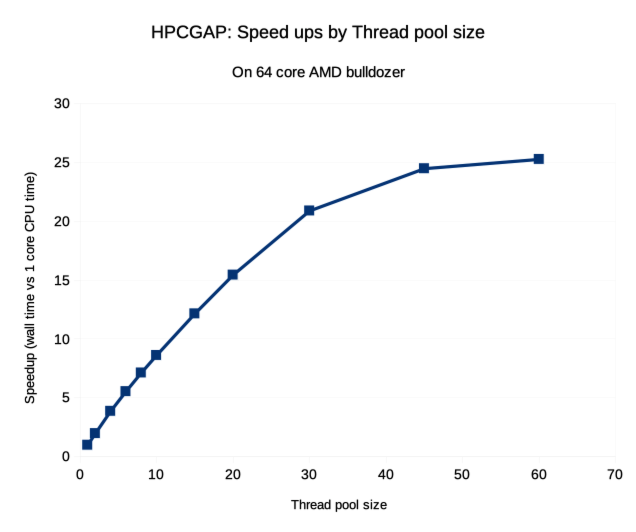
\includegraphics[width=0.8\textwidth]{images/hpcgap-speedups}
    \caption{Speedups achieved by HPCGAP on 1000 test tasks}\label{fig:hpcgap-speedups}
\end{figure}


% Release announcement: https://www.gap-system.org/Manuals/doc/changes/chap3.html#X7F52B77B7DBACC17

% \HPCGAP manual: https://www.gap-system.org/Manuals/doc/hpc/chap0.html

% What about making https://www.gap-system.org/Manuals/doc/hpc/manual.pdf 
% an electronic appendix to the deliverable?

\subsection{MeatAxe64: High-Performance Linear Algebra over Finite Fields}\label{meataxe64}

A key kernel for many applications of \GAP is linear algebra for
mainly dense matrices over
a range of finite fields, especially small ones. This is used directly in working with
matrix groups and in computational representation theory, but also
arises indirectly in areas such as graph theory, finite solvable
groups and number theory. 

The \GAP kernel already includes memory-efficient
representations of matrices over these fields, and implementations
based on the \software{C-MeatAxe} (the name ``MeatAxe'' is derived from the
abbreviation ``mtx'' for ``matrix'' and the fact that a key operation
in computational representation theory is to ``chop'' a module into
its irreducible components).

Working with external collaborators (primarily R.~A.~Parker), we have
supported (and continue to contribute to) the design and development
of a new C and assembler library, called \software{MeatAxe64}, which takes
advantage of new algorithmic ideas, and of powerful features of modern
CPUs, to deliver a quantum leap in performance for matrix
multiplication and Gaussian elimination on modern multi-core shared
memory computers. This project has involved radical innovations in
low-level data formats and arithmetic algorithms, in cache-friendly
loop structures (similar to those now standard in BLAS implementations,
but made more complex by the need to reorganize and reformat both
inputs and outputs of a multiplication), in matrix level reduction
algorithms (both for non-prime fields of all characteristics, inspired
by Albrecht \cite{m4rie}, and along Strassen-Winograd lines), in a
very efficient dataflow-driven thread farm and in high-level
algorithms, especially for Gaussian elimination. A number of
publications are in preparation.

We have implemented a \GAP interface to this C library (the
\software{MeatAxe64} \GAP package \cite{meataxe64}) currently in beta-testing,
and are in the process of revising higher levels of the software stack
to make best use of it.

The \software{MeatAxe64} C library is multi-threaded using a bespoke and
effective thread-farm that supports a powerful dataflow module of
computation. With this, the library can efficiently make
use of multiple cores for large enough matrices, whether used from
\HPCGAP or single-threaded \GAP. Particular care is taken to limit the use of
shared caches and of memory bandwidth in each task, so that they
interfere as little as possible. 

Tables \ref{fig:matmult:gap}, \ref{fig:matmult:mtx64} and
\ref{fig:matmult:par} indicate the performance gains and
speedups obtained by \software{MeatAxe64} compared to our existing code.  The
data is based on run-times for multiplication of two random dense
square matrices of the given dimension with entries from $GF(q)$. In
these tables the throughput is calculated as the cube of the dimension
divided by the elapsed (``wall-clock'') time, ignoring algorithmic
techniques that may reduce the actual number of field operations
needed. The unit (Gfop/s) is billions of field operations per
second. 


\begin{small}
\begin{center}  
  \begin{longtable}{|c|c|c|c|c|}
\caption[]{Performance of existing \GAP code}\label{fig:matmult:gap}\\
    \hline
    $q$&Dim.&cpu (s)&wall (s) &throughput\\
    &&&& (Gfop/s)\\
    \hline
    \endfirsthead
\caption[]{Performance of existing \GAP code}\\
    \hline
    $q$&Dim.&cpu (s)&wall (s) &throughput\\
    &&&& (Gfop/s)\\
    \hline
    \endhead
    \hline
    \endfoot
2&800&0.004&0.003&149.6\\
2&1600&0.016&0.016&255.8\\
2&4000&0.159&0.159&401.7\\
2&8000&1.581&1.582&323.6\\
2&16000&14.241&14.280&286.8\\
2&40000&193.251&193.524&330.7\\
3&500&0.053&0.052&2.4\\
3&1000&0.364&0.364&2.8\\
3&2500&5.268&5.268&3.0\\
3&5000&41.529&41.533&3.0\\
3&10000&327.798&328.121&3.0\\
3&25000&5020.887&5025.466&3.1\\
4&400&0.017&0.017&3.8\\
4&800&0.112&0.112&4.6\\
4&2000&1.542&1.542&5.2\\
4&4000&12.107&12.108&5.3\\
4&8000&99.259&99.361&5.2\\
4&20000&1513.64&1515.528&5.3\\
5&300&0.021&0.021&1.3\\
5&600&0.147&0.148&1.5\\
5&1500&2.166&2.166&1.6\\
5&3000&17.106&17.108&1.6\\
5&6000&136.714&136.840&1.6\\
5&15000&2088.063&2089.934&1.6\\
7&200&0.009&0.009&0.9\\
7&400&0.063&0.062&1.0\\
7&1000&0.906&0.906&1.1\\
7&2000&7.32&7.321&1.1\\
7&4000&56.659&56.710&1.1\\
7&10000&875.08&875.901&1.1\\
16&200&0.007&0.007&1.2\\
16&400&0.044&0.044&1.4\\
16&1000&0.644&0.643&1.6\\
16&2000&4.978&4.978&1.6\\
16&4000&39.757&39.798&1.6\\
16&10000&628.858&629.651&1.6\\
17&100&0.003&0.003&0.4\\
17&200&0.018&0.018&0.4\\
17&500&0.273&0.273&0.5\\
17&1000&2.153&2.154&0.5\\
17&2000&17.119&17.131&0.5\\
17&5000&268.032&268.267&0.5\\
64&100&0.002&0.002&0.5\\
64&200&0.012&0.013&0.6\\
64&500&0.186&0.186&0.7\\
64&1000&1.448&1.448&0.7\\
64&2000&11.548&11.558&0.7\\
64&5000&294.897&297.453&0.4\\
81&100&0.003&0.003&0.4\\
81&200&0.019&0.019&0.4\\
81&500&0.284&0.284&0.4\\
81&1000&2.215&2.215&0.5\\
81&2000&21.285&21.353&0.4\\
81&5000&276.045&276.503&0.5\\
101&100&0.003&0.003&0.3\\
101&200&0.021&0.020&0.4\\
101&500&0.295&0.295&0.4\\
101&1000&2.287&2.287&0.4\\
101&2000&18.212&18.233&0.4\\
101&5000&321.134&322.902&0.4\\
  \end{longtable}
\end{center}

\begin{center}
  \begin{longtable}{|c|c|c|c|c|}
    \caption[]{Performance of \software{MeatAxe64} on one core}\label{fig:matmult:mtx64}\\
    \hline
    $q$&Dim.&cpu (s)&wall (s) &throughput\\
    &&&&(Gfop/s)\\
    \hline
    \endfirsthead
    \caption[]{Performance of \software{MeatAxe64} on one core}\\
    \hline
    $q$&Dim.&cpu (s)&wall (s) &throughput\\
    &&&&(Gfop/s)\\
    \hline
    \endhead
    \hline
    \endfoot
2&8000&0.478&0.490&1045.1\\
2&16000&3.476&3.541&1156.7\\
2&40000&47.125&47.713&1341.4\\
2&80000&327.569&331.744&1543.4\\
2&160000&3460.336&3522.279&1162.9\\
3&5000&0.566&0.578&216.3\\
3&10000&4.125&4.152&240.9\\
3&25000&56.788&56.971&274.3\\
3&50000&399.282&400.549&312.1\\
3&100000&2774.011&2798.002&357.4\\
4&4000&0.205&0.216&295.8\\
4&8000&1.475&1.480&346.0\\
4&20000&19.889&20.070&398.6\\
4&40000&140.18&141.497&452.3\\
4&80000&980.936&985.148&519.7\\
5&3000&0.585&0.588&45.9\\
5&6000&4.102&4.107&52.6\\
5&15000&53.351&53.394&63.2\\
5&30000&362.048&362.369&74.5\\
5&60000&2585.863&2589.959&83.4\\
7&2000&0.217&0.221&36.2\\
7&4000&1.541&1.545&41.4\\
7&10000&20.652&20.675&48.4\\
7&20000&145.626&145.854&54.8\\
7&40000&1014.896&1016.415&63.0\\
16&2000&0.085&0.089&89.7\\
16&4000&0.603&0.623&102.7\\
16&10000&8.538&8.625&115.9\\
16&20000&60.979&61.521&130.0\\
16&40000&426.445&430.764&148.6\\
17&1000&0.074&0.074&13.5\\
17&2000&0.51&0.510&15.7\\
17&5000&7.259&7.265&17.2\\
17&10000&50.043&50.081&20.0\\
17&20000&352.604&353.215&22.6\\
64&1000&0.034&0.038&26.0\\
64&2000&0.201&0.206&38.7\\
64&5000&2.57&2.604&48.0\\
64&10000&17.858&18.125&55.2\\
64&20000&125.306&127.344&62.8\\
81&1000&0.095&0.099&10.1\\
81&2000&0.492&0.497&16.1\\
81&5000&5.519&5.560&22.5\\
81&10000&39.363&39.592&25.3\\
81&20000&274.394&276.197&29.0\\
101&1000&0.107&0.108&9.3\\
101&2000&0.75&0.751&10.7\\
101&5000&10.374&10.385&12.0\\
101&10000&72.007&72.056&13.9\\
101&20000&507.043&507.795&15.8\\
  \end{longtable}
\end{center}
  
\begin{center}
  \begin{longtable}{|c|c|c|c|c|}
    \caption[]{Performance of \software{MeatAxe64} on 64 cores}\label{fig:matmult:par}\\
    \hline
    $q$&Dim.&cpu (s)&wall (s) &throughput\\
    &&&&(Gfop/s)\\
    \hline
    \endfirsthead
    \caption[]{Performance of \software{MeatAxe64} on 64 cores}\\
    \hline
    $q$&Dim.&cpu (s)&wall (s) &throughput\\
    &&&&(Gfop/s)\\
    \hline
    \endhead
    \hline
    \endfoot
2&80000&904.369&21.638&23662.2\\
2&160000&4638.836&151.735&26994.4\\
2&320000&33340.649&1040.551&31491.0\\
3&50000&1004.631&21.017&5947.6\\
3&100000&5443.318&196.317&5093.8\\
3&200000&39283.76&1201.458&6658.6\\
4&40000&355.516&10.157&6300.9\\
4&80000&2548.595&51.267&9987.0\\
4&160000&13560.306&538.945&7600.0\\
5&30000&974.333&18.874&1430.6\\
5&60000&6273.661&142.248&1518.5\\
5&120000&38362.156&1171.026&1475.6\\
7&20000&437.489&8.740&915.3\\
7&40000&3035.705&53.539&1195.4\\
7&80000&15050.673&465.735&1099.3\\
16&20000&89.048&7.138&1120.8\\
16&40000&1044.91&22.805&2806.4\\
16&80000&6212.503&202.530&2528.0\\
17&10000&141.266&2.999&333.4\\
17&20000&1001.397&17.793&449.6\\
17&40000&7038.438&123.414&518.6\\
64&10000&58.099&1.807&553.5\\
64&20000&342.525&8.892&899.6\\
64&40000&2310.548&45.095&1419.2\\
81&10000&120.235&2.640&378.7\\
81&20000&734.844&13.992&571.8\\
81&40000&4913.959&88.109&726.4\\
101&10000&216.491&4.269&234.3\\
101&20000&1508.308&26.374&303.3\\
101&40000&10572.959&182.572&350.5\\
  \end{longtable}
\end{center}
\end{small}

% Release is published last week. Added to the bibliography. -- AK
% Thanks. I'd like to add a release announcement somewhere. -- SL


\section{Developments in the Core \GAP System}\label{sec:core-gap}

This Section highlights some of the most important
changes to the core \GAP system released
during the project which contribute to \ODK goals. Other important developments are
included in \GAP packages and described in later sections.  More
detailed descriptions of each major and minor \GAP release, with links
to the corresponding source code changes on GitHub, are contained in
the ``GAP - Changes from Earlier Versions'' document. This document is
redistributed with \GAP and is also available on the \GAP web site at
\url{https://www.gap-system.org/Manuals/doc/changes/chap0.html} and
included as an Appendix~\ref{sec:changes-manual} to this report.

This work includes many contributions from collaborators outside \ODK,
whose authorship can be seen from the version control history.

\subsection{libGAP: Allowing 3rd Party Code to Link \GAP Efficiently as a Library}\label{libgap}

The initial connection between \Sage and \GAP was developed around
2006, and relied on running a full \GAP process with which \Sage
communicated through UNIX pipes, creating \GAP input as text and then parsing
the text which was output from \GAP. This enabled an initial connection, but
introduced considerable overhead converting objects to and from text
representations and passing them between processes, and considerable
unreliability, since \Sage was essentially using \GAP through an
interface designed for humans, rather than programs.

A better solution is to provide a C API enabling \GAP to be integrated
into the \Sage process, and allowing a \GAP session to be started,
objects created, functions called and results retrieved, via C function
calls. This is, however, not a mode of operation for which \GAP was
ever designed, and implementing it in a robust and flexible way
required considerable adaptations to the system, essentially
disentangling the computational engine from the user interface, while retaining,
for example, the ability to dynamically load C code from \GAP
packages into the process that was using {\sf libGAP}. Another complication
is the need to make sure that the \GAP memory manager does not delete
objects which the calling process will want in the future.

Based on an initial version developed within the \Sage team, a fully
general-purpose and flexible version was released in \GAP 4.10.0
(Month 39).

Subsequent releases have improved and will continue to improve the
robustness of libGAP, and to extend its API with new functionality
(For the detailed descriptions, see Chapter 2 
``Changes between \GAP 4.9 and \GAP 4.10'' of the 
``\GAP\,- Changes from Earlier Versions'' manual,
provided in Appendix~\ref{sec:changes-manual}).
This has allowed \Sage to drop its custom 
modifications to \GAP and use an official, documented and regularly 
tested \GAP interface instead, starting from SageMath 8.6 (Month 41).

% See SageTrac ticket 22626 made that happen; it was merged in 
% SageMath 8.6.beta0, so SageMath 8.6 had it but not SageMath 8.5.

\subsection{Linguistic Reflection -- Supporting Transformation and
  Optimisation of \GAP Functions at Runtime}\label{syntaxtree}
The \GAP programming language, in which much of the system is written,
is interpreted and dynamically typed (somewhat like the better-known
Python). It has a unique ``method selection'' system
(\cite{BreuerLinton98}) in which the type of an object reflects
mathematical information learned about it at runtime; method
selection uses the known types of all arguments in order to choose a method.

A compiler for the language (converting \GAP code
into C extensions to the \GAP kernel) has been available for many
years as part of \GAP, but gives surprisingly little speedup on most code, and has not
seen widespread adoption. The main reason for this is that objects'
types must still be checked, and method selection decisions made, at
run-time, even in compiled code.

\Sage, implemented initially in Python, faced many of the same
problems, and addressed them by adopting, and promoting
development of, the \href{http://cython.org}{Cython} project, which
extends the Python language with C-like types and constructions to
allow more effective compilation.

In WP5 the \GAP team have sought a natural and usable way to deliver
similar benefits for the \GAP language (bearing in mind the relative
sizes of the \GAP and Python user and developer communities). After
some experiments and a great deal of discussion across the community,
we have settled on ``Linguistic reflection'', combined with code
annotations (pragmas) as an approach that offered a good return of
performance and other benefits for the effort invested.

The key infrastructural tools for both of these have now been added to
the \GAP language and interpreter. The new \verb|SyntaxTree| function
``unpacks'' the workspace representation of a \GAP function,
converting it into a data structure which can be easily manipulated by
\GAP, and converted back into a new executable \GAP function when
needed. Code annotations in the form of pragmas are retained through
this process, so that the programmer can use them to guide in
program transformation, and different software transformers can use
them to communicate. All of this functionality is publicly available
now in the development version of \GAP on GitHub and will be included
in \GAP 4.11 (expected November 2019).

Future versions will build on this for optimization, OpenMP-style
semi-automatic parallelization and (our original motivating
application) to produce specialized versions of functions which reduce
the amount of run-time method selection required, allowing them to be
executed more quickly and compiled to C more effectively.

As a small example, consider the following code fragment:


\begin{Small}
\begin{verbatim}
foo := function(n, x, y)
    local z,i;
    z := 0;
    for i in [1..n] do
        #% x and y always integers
        z := z+Gcd(x,y);
    od;
    return z;
end;
\end{verbatim}
\end{Small}

The \verb|#%| here denotes a pragma. This can be unpacked to produce
the cumbersome, but easily processed data structure shown in Figure \ref{fig:syntaxtree}.

\begin{figure}[!ht]
  \begin{mdframed}
  \begin{Small}
\begin{verbatim}
gap> t:= SyntaxTree(foo)!.tree;
rec( name := "foo", nams := [ "n", "x", "y", "z", "i" ], narg := 3, 
  nloc := 2, 
  stats := 
    rec( 
      statements := 
        [ 
          rec( lvar := 4, rhs := rec( type := "EXPR_INT", value := 0 ), 
              type := "STAT_ASS_LVAR" ), 
          rec( 
              body := 
                [ 
                  rec( type := "STAT_PRAGMA", 
                      value := "% x and y always integers" ), 
                  rec( lvar := 4, 
                      rhs := 
                        rec( 
                          left := 
                            rec( lvar := 4, type := "EXPR_REF_LVAR" ), 
                          right := 
                            rec( 
                              args := 
                                [ 
                                  rec( lvar := 2, 
                                      type := "EXPR_REF_LVAR" ), 
                                  rec( lvar := 3, 
                                      type := "EXPR_REF_LVAR" ) ], 
                              funcref := 
                                rec( gvar := "Gcd", 
                                  type := "EXPR_REF_GVAR" ), 
                              type := "EXPR_FUNCCALL_2ARGS" ), 
                          type := "EXPR_SUM" ), 
                      type := "STAT_ASS_LVAR" ) ], 
              collection := 
                rec( first := rec( type := "EXPR_INT", value := 1 ), 
                  last := rec( lvar := 1, type := "EXPR_REF_LVAR" ), 
                  type := "EXPR_RANGE" ), type := "STAT_FOR_RANGE2", 
              variable := rec( lvar := 5, type := "EXPR_REF_LVAR" ) ), 
          rec( obj := rec( lvar := 4, type := "EXPR_REF_LVAR" ), 
              type := "STAT_RETURN_OBJ" ) ], type := "STAT_SEQ_STAT3" )
    , type := "EXPR_FUNC", variadic := false )
\end{verbatim}
  \end{Small}
  \end{mdframed}
  \caption{A Full Syntax Tree Data Structure}\label{fig:syntaxtree}
  \end{figure}
  

This data structure contains all of the necessary information for
a simple \GAP program to locate the pragma and, using the information
in it, replace the general function \verb|Gcd| by the specialized
\verb|GcdInt| statically.  Doing this by hand for the moment, we can
produce the session in Figure \ref{fig:using-syntaxtree}. This shows 
the full round trip from one executable \GAP function \verb|foo| to an
optimised one \verb|bar| which completes in approximately one fifth the time.

\begin{figure}[!ht]
  \begin{mdframed}
\begin{Small}
\begin{verbatim}
gap> foo := function(n, x, y)
>     local z,i;
>     z := 0;
>     for i in [1..n] do
>         #% x and y always integers
>         z := z+Gcd(x,y);
>     od;
>     return z;
> end;
function( n, x, y ) ... end
gap> t := SyntaxTree(foo)!.tree;;
gap> u := StructuralCopy(t);;
gap> u.stats.statements[2].body[1].value := "% Gcd specialised to GcdInt";;
gap> u.stats.statements[2].body[2].rhs.right.funcref.gvar := "GcdInt";;
gap> bar := SYNTAX_TREE_CODE(u);;
gap> Print(bar);
function ( n, x, y )
    local z, i;
    z := 0;
    for i in [ 1 .. n ] do
        #% Gcd specialised to GcdInt
        z := z + GcdInt( x, y );
    od;
    return z;
end
gap> foo(10^7, 102334155, 165580141);; time
2245
gap> bar(10^7, 102334155, 165580141);; time;
424
\end{verbatim}
\end{Small}
  \end{mdframed}
  \caption{An example of manual optimisation using pragmas and Syntax
    Trees}\label{fig:using-syntaxtree}
  \end{figure}
  

\textbf{Note:} It is important to understand that this is \emph{not} a
source code level transformation. Automated transformation tools built
on this foundation do
not need to parse or emit \GAP syntax, and all questions of scope,
including bindings in closures, are already resolved. A small planned
extension will add profiling information to the syntax tree when available.

Other applications for this technology include automated
parallelization (in combination with \HPCGAP) and traditional code optimizations.

While we would have preferred to have had more time to exploit these
facilities within the project, it was important to achieve consensus
around a solution that fit the needs of \GAP and its community and
will provide a basis for developments for years to come.

\subsection{Developments in \GAP 4.8 (Month 8)}\label{gap-4.8}

\GAP 4.8 was the first major release of \GAP published
after the start\footnote{In the report we
refer to months of the project, i.e. Month 1 is September 2015, while Month 48 is August 2019.}
of the \ODK project. 
In preparation for the planned integration of the \HPCGAP branch
(supporting \GAP language-level threading) into
the core system, some language extensions were backported to core
\GAP at this stage. 
This helped to unify the codebases of \GAP~4 and \HPCGAP
by allowing \HPCGAP code to be read in a single-threaded
\GAP session. For example, the
\verb|atomic|, \verb|readonly| and \verb|readwrite| keywords used for
controlling access to shared data in \HPCGAP were
added as ``no-ops'' to the regular \GAP language.


In addition, this release also provided support for much enhanced
profiling, essential to all our performance engineering work.
Previously, \GAP\ allowed tracking of the CPU time spent
executing each function, but the new features in this release
reduced this granularity to individual lines of \GAP
code. Related developments also made it easier to track time spent on
individual lines of C code in the \GAP kernel. A further related
feature makes it very easy to measure ``test coverage'' -- the
proportion of the system that has actually been executed by a given
set of tests. The {\sf Profiling} package \cite{profiling} by Christopher Jefferson
(USTAN) provided excellent tools for transforming these profiles into
various human-readable forms. These features supported later work on
enhancing both the performance and the reliability of \GAP, through
easier identification of hot-spots and easier measurement of test
quality.

This release also included some language extensions which would allow
users to write more efficient and readable code:

\begin{itemize}
  \item support for \emph{partially
  variadic functions} similar to those allowed in Python, allowing
function expressions like
\verb|function( a, b, c, x... ) ... end;|
which requires at least three arguments \verb|a|, \verb|b| and
\verb|c| and assigns the first three to \verb|a|, \verb|b| and \verb|c|
and then a list containing any remaining ones to \verb|x|.
\item more flexible list indexing, allowing users to install methods
  for multiple indexing (\verb|m[i,j]| instead of \verb|m[i][j]| for
  arrays) and more varied indices (such as \verb|l[-1]| to access a
  doubly-infinite virtual list \verb|l|). As well as being more
  flexible, this is a step towards supporting more efficient array
  implementations in which ``row objects'' (like \verb|m[i]| in
  \verb|m[i][j]|) might not exist.
\end{itemize}

\GAP 4.8 had seven public releases between Month 6 and Month 24, and
was replaced by \GAP 4.9 in Month 33.

\subsection{Developments in \GAP 4.9 (Month 33)}\label{gap-4.9}

\GAP 4.9 continued the restructuring and modernizing of the core \GAP
system, aiming at the greater reliability, flexibility and performance
which would be needed for \GAP users to gain the full advantage of the \ODK ecosystem.
For example, we removed our old home-grown large integer arithmetic
implementation, and committed fully to the state of the art external
library \href{???}{GMP}. This
move continues our cautious programme of exploiting existing free
software in our core system. Our caution here is based on
experience. Moving too quickly in this area in the past has created
problems with the reliability and
portability of \GAP on which our users depend.

This release incorporated a completely
reimplemented build system for \GAP, using more modern tools and
complying with modern expectations. This resolved many issues with the
old system, and made it easier to maintain and extend. For example it
makes it much easier to maintain multiple configurations of \GAP on a
single system from a single copy of the source. Technical
details of the new build system are described in {\tt
  README.buildsys.md} from the \GAP source code. Crucially the new build system
was the final prerequisite for the planned  merge of the \HPCGAP codebase  into the
mainstream \GAP system as a compile-time option (for details, see
Subsection~\ref{hpc-gap}).

An additional benefit of the new build system is that it makes it much
easier to robustly include C or C++ extensions to the \GAP kernel in
contributed packages, including interfaces to many free C and C++
libraries. By making it easy to accelerate bottleneck steps, this
greatly enhanced the overall performance of many packages, while
encouraging integration of existing C libraries in packages complements
our cautious approach mentioned above to including them in the core
system.

One such example is the {\sf Semigroups} package \cite{Semigroups} by James D.
Mitchell (USTAN).  This started as a pure \GAP package not requiring compilation,
but a number of key algorithms from it were later converted into C and C++ in
order to achieve the high performance necessary for its use in mathematical
research.  Rather than keeping these algorithms in a simple \GAP kernel
extension, they were made into a separate C++ library called {\sf libsemigroups}
\cite{libsemigroups}, which does not rely on \GAP or any of its packages.  This
library is a required component of the {\sf Semigroups} package, and provides
high-performance code to compute such objects as presentations, Cayley graphs
and rewriting systems for finite semigroups, as well as information about
semigroup congruences.  Many parts of the library support multi-threading,
meaning that users with multi-core computers can take advantage of parallelism
even when not running \HPCGAP.  Furthermore, the library can be accessed from
Python or \Sage via \href{https://github.com/libsemigroups/libsemigroups-python-bindings}{a special set of Python bindings}
 without
any need for \GAP to be loaded.  The development of these bindings, other work
on {\sf libsemigroups}, and the mathematical research that came from it, are
good examples of \ODK collaboration between USTAN and UPSud.
An example of {\sf libsemigroups} being called and used through \GAP is shown in
Appendix~\ref{sec:libsemigroups-notebook}.

Another example is the {\sf curlInterface} package \cite{curlInterface}
by Christopher Jefferson and Michael Torpey, which first appeared
in \GAP 4.9.3 distribution.  This package allows a user to interact 
with http and https servers on the Internet, using the {\sf curl} library, 
and is used by the {\sf PackageManager} package
\cite{PackageManager} described in Subsection~\ref{pkg-manager}.

The \GAP~4.9.1 release also incorporated the new {\sf ZeroMQInterface}
package
\cite{ZeroMQInterface} by Markus Pfeiffer and Reimer Behrends, which
provides both low-level bindings as well as some higher level interfaces
for the {\sf ZeroMQ} message passing library for \GAP and \HPCGAP, 
enabling lightweight distributed computation. 


The release of this package at this time allowed us to include in \GAP~4.9.2 a
further three packages.  Firstly we have the {\sf JupyterKernel} package \cite{JupyterKernel} 
by Markus Pfeiffer, developed under WP4 and reported in deliverable D4.7,
providing a so-called kernel for the
\href{https://jupyter.org/}{Jupyter interactive document system}. This package
requires GAP packages {\sf IO}, {\sf ZeroMQInterface}, {\sf json},
and also two other new packages by Markus Pfeiffer called
{\sf crypting} and {\sf uuid} \cite{crypting,uuid}, all included 
in the \GAP~4.9.2 distribution.

\GAP~4.9.3 also included the {\sf datastructures} package \cite{datastructures}
by Markus Pfeiffer, Max Horn, Christopher Jefferson and Steve Linton, which aims 
at providing standard datastructures, consolidating existing code and improving 
on it, in particular in view of \HPCGAP.

The \GAP~4.9.1 release also incorporated many smaller performance improvements. For example,
\GAP now supports named constants, whose value cannot change 
at runtime. While maintaining readability through naming, uses of
these constants can be optimized as a function is parsed, so that they
are at least as fast as using explicit values. Another notable improvement was
to the widely used  sorting functions which now use the best
recently published algorithms and were also made easier to maintain by
restructuring the implementation.

Debugging  and profiling tools were also improved based on experience with
\GAP 4.8. Further changes improved \GAP
usability by allowing more efficient and/or readable code, in line
with other modern programming languages:
\begin{itemize}
  \item a concise syntax for short
    functions with any number of arguments, so that, for example,
    \verb|{a,b} -> a+b| abbreviates \verb|function(a,b) return a+b; end|. 
\item more flexibility in \GAP expression syntax,
  where previously there were unintuitive technical restrictions. For
  example, an entry of the sum of two vectors can now be accessed as
  \verb|x := (v+w)[i]| instead of \verb|u := v+w; x := u[i]|.
  
%%   use of function literals in expressions such \verb|y := f().x;|
%% replacing previously required two-step calculation
%% \verb|y := f();; y := y.x;|.
%% This -- and the release
%%   announcement -- are actually wrong! This syntax always worked, the
%%   example in the PR is \verb|(f()).x| which is different}

\end{itemize}

\GAP 4.9 had three public releases between Months 33 and 37, and
was replaced by \GAP~4.10 in Month 39.

\subsection{Developments in \GAP 4.10 (Month 39)}\label{gap-4.10}

The release of \GAP 4.9 with the new build system allowed the
restructuring of the core \GAP system to continue, and allowed us to
finalize a number of other ongoing changes, leading to \GAP 4.10
after a shorter-than-usual interval. \GAP 4.10 is the current
version of \GAP, with the latest release being \GAP 4.10.2, published
in Month 46, and \GAP 4.11 expected in November 2019.

The most important new feature in \GAP 4.10 was the first public
release of {\sf libGAP}: an
option to compile \GAP as a C library instead of a stand-alone
executable. This is very important for many uses of \GAP in \ODK and
was discussed in further detail in Section \ref{libgap} below.

\GAP 4.10 also provides experimental support for using alternative
memory management systems, notably the \href{https://julialang.org/}{Julia} garbage
collector and the \href{http://www.hboehm.info/gc/}{Boehm garbage collector}, in place of the
GASMAN system which was developed for \GAP 4 in the 1990s.  These
garbage collectors are thread-safe (important for \HPCGAP) and the
option to use the Julia garbage collector will allow tight integration
of \GAP with Julia programs and other systems via Julia. Use of Julia
in this way is an initiative led by the
\href{https://oscar.computeralgebra.de/}{OSCAR} project, developed
within the DFG-funded grant SFB-TRR 195 ``Symbolic Tools in
Mathematics and their Application'' and is seen as complementary to \ODK.

The work on improving debugging and profiling in \GAP has
continued. Profiling now reports memory usage as well as CPU time, and
additional checking options (both internal and by using external tools such as
\href{http://www.valgrind.org/}{valgrind}) help to detect misuse of memory in the kernel.

Using the improved debugging and profiling facilities we were able to
detect many performance bottlenecks and confirm that new code
genuinely improved performance, as well as detecting many bugs much
earlier in the development process. To alleviate performance
bottlenecks in key applications, we rewrote much of the method
selection (dispatch) code from \GAP to C and gained large speedups by
re-engineering many integer arithmetic functions.

For example, the table below gives the CPU time in milliseconds required
to run the following calculation:

\begin{verbatim}
for i in [1..k] do x:= 1/p^q mod n; od;
\end{verbatim}
\medbreak
\begin{center}
\begin{tabular}{| c | c | c | c | c | c |} 
\hline
p & q    & n          & k        & ms, before & ms, after \\
\hline
3 & 60   & $2^{59}$   & 2000000  & 2364       & 1219 \\
3 & 60   & $2^{60}$   & 2000000  & 2821       & 1292 \\
2 & 6000 & $3^{6000}$ & 6000     & 19358      & 692  \\
\hline
\end{tabular}
\end{center}

%Before
%gap> q:=1/3^60;;n:=2^59;; for i in [1..2000000] do x:= q mod n; od; time;
%2364
%gap> q:=1/3^60;;n:=2^60;; for i in [1..2000000] do x:= q mod n; od; time;
%2821
%gap> q:=1/2^6000;;n:=3^6000;; for i in [1..6000] do x:= (q mod n); od; time;
%19358
%
%After:
%
%gap> q:=1/3^60;;n:=2^59;; for i in [1..2000000] do x:= q mod n; od; time;
%1219
%gap> q:=1/3^60;;n:=2^60;; for i in [1..2000000] do x:= q mod n; od; time;
%1292
%gap> q:=1/2^6000;;n:=3^6000;; for i in [1..6000] do x:= (q mod n); od; time;
%692

%\TODO{Maybe drop this next one, a bit technical? AK: maybe (mention only last
%line maybe - enables calculation not easily doable in default memory settings before?}
%
%Also, \verb|InverseMatMod| with integer modulus has been improved.% #2426
%The following table shows the runtime needed to call
%\verb|x:=InverseMatMod(m,q);| a hundred times for a random unimodular $100 \times 100$
%matrix \verb|m|:
%
%\begin{center}
%\begin{tabular}{| c | c | c |} 
%\hline
%q     & ms, before    & ms, after \\
%\hline
%2     & 277           & 273 \\
%251   & 1564          & 1249 \\
%65537 & out of memory & 1226 \\
%\hline
%\end{tabular}
%\end{center}

%Before:
%
%gap> m2:=RandomUnimodularMat(100);;
%gap> for i in [1..100] do x:=InverseMatMod(m2,2); od; time;
%277
%gap> for i in [1..100] do x:=InverseMatMod(m2,251); od; time;
%1564
%gap> for i in [1..100] do x:=InverseMatMod(m2,65537); od; time;
%Error, reached the pre-set memory limit
%
%After:
%
%gap> m2:=RandomUnimodularMat(100);;
%gap> for i in [1..100] do x:=InverseMatMod(m2,2); od; time;
%273
%gap> for i in [1..100] do x:=InverseMatMod(m2,251); od; time;
%1249
%gap> for i in [1..100] do x:=InverseMatMod(m2,65537); od; time;
%1226

The same improved profiling tools identified other
``hidden'' bottlenecks in \GAP code. For instance \GAP has a
sophisticated system of inference that can trigger 
so-called ``immediate methods'': quick attempts to deduce additional
consequnces from information that becomes known about an object.
In general, these are very effective, and the deduced information can
lead the system to chose better methods for subsequent
calculations. For instance, when a group learns its order, if that
order is finite and odd, then by the celebrated
Feit--Thomson theorem the group must be solvable. Once that
is known, much more efficient methods can be applied for many
subsequent calculations.

While this is a powerful feature in most situations, in some
calculations, a large number of short-lived objects are created,
and the immediate methods use a great deal of time deducing knowledge
about each of them
that will never be used. The profiling developments made this 
easily visible for the first time, and some small adjustments to the
immediate methods produced up to a six-fold speed-up in fundamental
operations such as computing isomorphism groups. For instance, the
run-time for the code fragment below dropped from 130
seconds to 22.


{\Small
\begin{verbatim}
G:=PcGroupCode( 
  741231213963541373679312045151639276850536621925972119311,
  11664);;
IsomorphismGroups(G,PcGroupCode(CodePcGroup(G),Size(G)))<>fail;
\end{verbatim}
}


We have also continued to develop package {\sf JupyterKernel} following 
its inclusion in \GAP~4.9 to enhance its usability. The advent of
\href{https://mybinder.org/}{Binder} allowed us to give users an
opportunity to try \GAP Jupyter notebooks online 
and share reproducible \GAP experiments (see Appendix~\ref{sec:repro-gap}).

The inclusion of the {\sf JupyterKernel} package and its associated 
dependencies into \GAP~4.9 facilitated the appearance of new packages
extending its graphical capabilities. \GAP 4.10.0 incorporated 
the {\sf Francy} package \cite{Francy} by Manuel Martins and
the {\sf JupyterViz} package \cite{JupyterViz} by 
Nathan Carter\footnote{Nathan Carter visited USTAN on sabbatical from
Bentley University in 2018--2019, and was employed part time to work
mainly on WP3. In addition to {\sf JupyterViz}, he also carried out a major redesign
of his {\sf GroupExplorer} software -- a popular teaching resource, 
accompanied by the textbook \cite{Carter-book}, which had been developed
in the previous decade and was in an
urgent need of modernization. The new {\sf GroupExplorer} version, available
at \cite{GroupExplorer}, also allows a user to load and run the \GAP code
to construct and explore groups from the {\sf GroupExplorer} library
interactively, launching a \GAP session on a \SageMath cell server.
}
which allow users to create and work with charts and graphs. The latter
package also allows the user to produce graphics from the \GAP command line.


\subsection{Developments in \GAP 4.11 (anticipated in November 2019)}\label{gap-4.11}

% Since they are released on GitHub, I see no reason not to also
% highlight changes which are merged and definitely coming out in
% 4.11, if they are relevant SL

% Release notes are collected at https://github.com/gap-system/gap/wiki/GAP-4.11-release-notes

At the time of preparation of this report, the next major release,
\GAP~4.11,
is approaching completion. Almost all of the features to be
included in it (including all the ones highlighted here) are already
publicly  available on GitHub to developers or anyone else interested.

One important and relevant feature of this release will be the ``syntaxtree'' reflection
API for \GAP, allowing \GAP programs to access and modify the internals of \GAP
functions and opening up a range of possibilities for optimization, automatic
parallelization, and more effective compilation into C. This is
discussed in more detail in Section \ref{syntaxtree} above. 

Additional relevant features are continued improvements to debugging and
profiling facilities (for example,
%#2772 
adding support for profiling interpreted code
and 
%#3420
making profiling reports more informative by 
giving more library methods human-readable names;
%#2900 %#1633 
and enhancements to the testing infrastructure designed to make the
test suite more robust and easier to run, and tests more independent
and easier to write).

The {\sf libGAP} API has been extended
to allow programs using the system in this way
more convenient access to \GAP objects such as
%#2998, #2999, #3007 
characters, floats, integers
%#3554
and matrices; 
%#3516
the performance of Julia GC integration also improved,
%#3335 
and the memory usage on Windows when running external programs was reduced.

Further performance enhancements included, among others,
%#3579 
speeding up writing to global variables;
%#3566 
optimizing operations involving identity permutations;
%#3231 
speeding up \verb|IsConjugate| for \verb|IsNaturalSymmetricGroup|,
%#2924 
improving performance of \verb|NormalizerViaRadical|,
%#3031 
and of \verb|ConjugacyClasses| for solvable groups. For example, the time
of the following calculation reduces from 110 seconds to 53 seconds:

{\Small
\begin{verbatim}
G:=WreathProduct(CyclicGroup(IsPermGroup,12),
       DihedralGroup(IsPermGroup,12));
ConjugacyGlasses(G);
\end{verbatim}
}
\noindent

% What about making pages for relevant releases in
% https://www.gap-system.org/Manuals/doc/changes/manual.pdf 
% (or print HTML version of the manual into PDF)
% an electronic appendix to the deliverable?
%
% Yes -- let's do that. Add them as appendices.
%
% Indeed, as the ODK README.md says:
%
%  The report shall be self-contained. Indeed, the
%  deliverable will be evaluated based upon its version submitted on
%  the EU portal without retrieving other resources. Links have no
%  legal value, since there is no guarantee that the referenced
%  material will remain unchanged. One may typically want to add
%  relevant material as appendix (e.g. snapshots of software
%  documentation, websites, or other relevant documents); see e.g.
%  [WP5/D5.1/report.tex](WP5/D5.1/report.tex) or
%  [WP2/D2.1/report.tex](WP2/D2.1/report.tex).


%% \comment{tests from 4.7.9 take 3237s in GAP 4.7.9;
%% 4.10.2: total 3039s (150s GC) and 328GB allocated;
%% GAP master: total 2913s (140s GC) and 293GB allocated}

As one example of the general effectiveness of our performance
improvements, the full test suite of \GAP 4.7.9 (current at the
start of the project) which takes 3237 seconds to run on \GAP 4.7.9 on
current hardware, runs unchanged in just over 2900 seconds with a
pre-release version of \GAP 4.11. Many of the most widely used and
important areas of \GAP functionality have seen bigger changes.  



\section{Additional Developments in \GAP packages} \label{sec:packages}

Other sections of this report describe
a number of \GAP packages such as Meataxe64 and Profiling that were developed, published,
and/or added to the \GAP distribution over the duration of the project.  In this section
we briefly list some other notable new or improved packages that
contribute to our overall goals of making \GAP more efficient, usable,
composable and scalable, and enabling users to solve larger and more
complex problems.

\begin{itemize}

\item
{\sf datastructures} \cite{datastructures} by Markus Pfeiffer, Max Horn, 
Christopher Jefferson and Steve Linton, which provides high
performance scalable implementations of modern standard datastructures
suitable for use in multi-threaded computations. (added in \GAP~4.9.3).
\TODO{is this one already covered in the section on \GAP 4.9?}

\item
{\sf Digraphs} by Jan De Beule, Julius Jonu\v{s}as, James Mitchell,
Michael Torpey and Wilf Wilson, which provides very efficient C-based
functionality for fundamental computations with directed and
undirected graphs, including those with multiple edges. (added in
\GAP~4.8.2 and repeatedly extended).  These algorithms underpin many
mathematical computations, especially in semigroups and combinatorics.

\item
{\sf ferret}  by Christopher Jefferson, which provides a C++
reimplementation of Jeffery Leon's Partition Backtrack framework for
solving graph-isomorphism like problems in permutation groups
(published as a package submitted for the redistribution with
\GAP). This has the effect of accelerating many standard
group-theoretic computations.

\item
{\sf FinInG} by John Bamberg, Anton Betten, Philippe Cara, Jan De
Beule, Michel Lavrauw and Max Neunh\"offer for computation in Finite
Incidence Geometry (added in \GAP~4.8.2).

\item
{\sf MajoranaAlgebras} by Markus Pfeiffer and Madeleine Whybrow, which
constructs Majorana representations of finite groups (added in
\GAP~4.10.1). This is interesting primarily as an application of high
performance kernels. This whole area of mathematics was inspired by
the Griess algebra used to construct the celebrated ``Monster''
sporadic simple group, which has dimension 196884. Many of the
interesting problems in this area has similarly high dimension and
\HPCGAP and meataxe64 methods have both been used to good effect in
this area.
%
% Possible demo?
%

\item
{\sf matgrp}  by Alexander Hulpke, which provides an interface
to the solvable radical functionality for matrix groups, building on
constructive recognition (added in GAP 4.8.2). This improves the
general capabilities of \GAP in this area, and reduces many key
problems to linear algebra and/or partition backtrack questions, which
can exploit the power of meataxe64 and/or ferret.

\item
{\sf NormalizInterface}  by Sebastian Gutsche, Max Horn and
Christof S\"oger, which provides a GAP interface to Normaliz, enabling
direct access to the complete functionality of Normaliz, such as efficient
computations in affine monoids, vector configurations, lattice
polytopes, and rational cones (added in GAP 4.8.2). 

\item
{\sf walrus} by Markus Pfeiffer, providing methods for proving 
hyperbolicity of finitely presented groups in polynomial time
(added in GAP 4.10.1). This again is an application area for High
Performance methods in \GAP, requiring some very unusual data
structures and search primitives.

\item
{\sf YangBaxter} by Leandro Vendramin and Alexander Konovalov, 
which provides functionality to construct classical and 
skew braces, and also includes a database of classical 
and skew braces of small orders (added in GAP 4.10.1).

\end{itemize}


\section{Developments in \GAP infrastructure: Tools and Processes for
  System and Package Development, Quality Assurance and Release }\label{sec:gap-infra}

As well as developments in the core system and in packages, we have
dedicated considerable effort to improving our infrastructure and
processes.  In this section we describe developments in the technical
processes which support our developers (especially package
developers). These processes connect developers to our user community and aim to ensure the
robustness and quality of the integrated system, something essential
to its use in demanding large-scale computations. Some of the
technical developments (especially around continuous integration) were
reported in D3.8 (Month 36), and some of the associated advocacy,
training and support in deliverables D2.2, D2.11 and D2.15. This
section updates and extends those focused reports, taking a broad
view of our tools and processes and focusing on the visible benefits
of these changes to developers and package authors. In subsection
\ref{sec:uptake} we assess the impact that this work has
had on the developers and package authors.

\subsection{Regression Testing}\label{testing}

\emph{Regression testing} %is a software engineering technique which
checks (preferably in an automated way)
that changes and additions to a system do not break functionality that 
worked previously. If a change breaks a test, that is 
a \emph{regression}. In \GAP, regressions may occur
when a change causes an incorrect result, or a crash, or an unwanted error
message; in addition, there may be \emph{performance regressions}
and \emph{memory regressions} where a test becomes slower, or uses
much more memory after a change.

Regression testing has been used by \GAP in one or another form since 
1980s, and by the beginning of the \ODK project, \GAP had established its testing infrastructure
based on a private \href{https://jenkins.io/}{\sf Jenkins} installation
at USTAN, not accessible outside the local network. That was a major limitation,
because sharing test outcomes with other developers and
allowing them to repeat tests in the same environment was cumbersome
and time-consuming with many manual steps.

%\GAP developers came to an understanding 
%that one of the limiting factors (not only for the testing, but for
%the \GAP development in general) was that while \GAP is an open source 
%software, it does not follow an open development model and does not
%have a public source code repository, and just before the start of
%the project established a public source code repository for \GAP
%on GitHub at \url{https://github.com/gap-system/gap}. 

%In the duration of the OpenDreamKit project we, together with other
%contributors to the \GAP project, consolidated \GAP development 
%around GitHub and its tool ecosystem.
%Hosting GAP repository on GitHub and eventual establishing of a number
%of other repositories under the gap-system and gap-packages 
%organizations (\url{https://github.com/gap-system} and 
%\url{https://github.com/gap-packages}), and encouraging package authors 
%to follow the same practices (see \url{https://gap-packages.github.io/})
%to find some further packages that are having public source code 
%repositories elsewhere) allowed us to bring our regression testing
%up to the next level.
%
%\TODO{maybe mention that we can break out onto GitLab if GitHub
%changes in some unacceptable way} 
%

During \ODK there has been widespread adoption of open development models by the
\GAP system and package developers and
maintainers. As a result, we have also been able to move
to an open regression testing infrastructure, which has enabled us
to substantially improve \GAP development and testing workflows and
develop a more robust system with less effort. For example,
today, anyone who is interested in checking the
status of the \GAP test suite can visit the public dashboard at
\url{https://github.com/gap-system/gap-distribution/} of which a
snapshot is shown in figure~\ref{fig:gap-core-tests}.
This dashboard shows the status of the core system GAP tests,
which are run for every change made to the repository, as well as
package integration tests described below.

\begin{figure}[!ht]
    \centering
    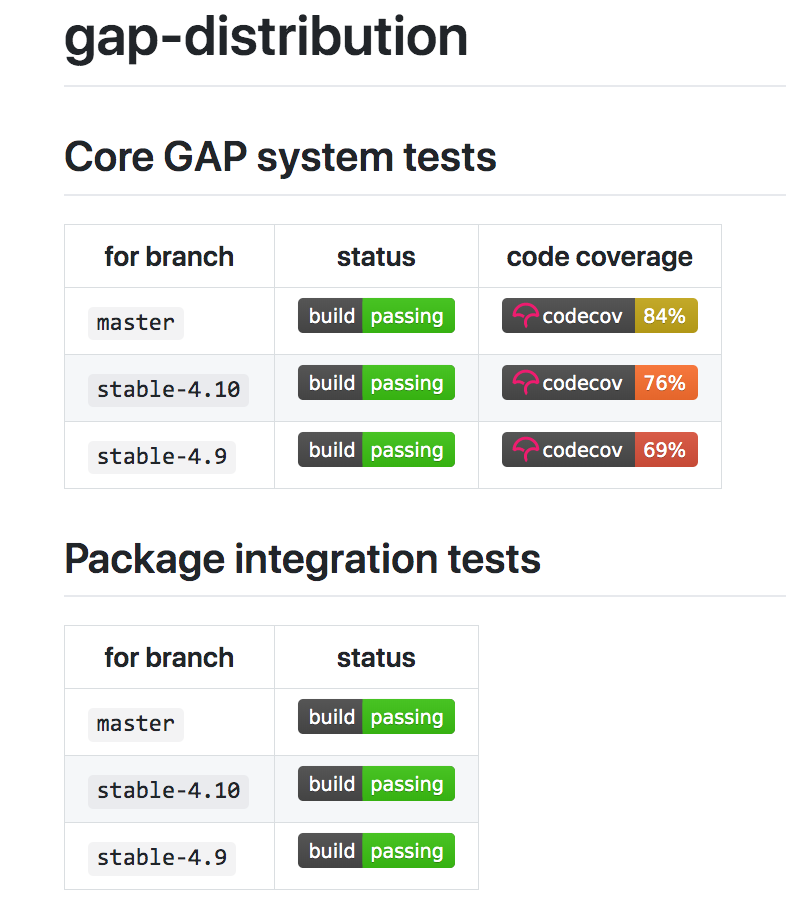
\includegraphics[width=5cm]{images/gap-core-tests}
    \caption{Dashboard with core GAP system and package integration tests}
    \label{fig:gap-core-tests}
\end{figure}


The ``status'' lights are actually active buttons, which lead to the
full test reports, held on the public continuous integration platform
\href{https://travis-ci.org/}{Travis CI}. The the ``code coverage''
lights are also buttons and lead to the public
\href{https://codecov.io/}{Codecov} service, where, if you drill down far
enough, you can access reports showing exactly which lines of code in the kernel
and library have, or have not been tested.

This level of open continuous testing has led to huge improvements in
the quality of the system, with far fewer bug reports than previously,
and saved enormous effort in integrating releases.

At the heart of the testing of the core \GAP system is our
comprehensive test suite. The table in
figure~\ref{fig:test-suite-growth} shows its increase over the period.
In addition, we also test the correctness of the
over $14,000$ lines in the 1810 examples in our manuals. We promote a similar testing approach to \GAP package authors and
encourage them to provide their own regression
tests. Many do, adding, in total over a quarter of a million lines of
further tests in the distributed system, which are run when new
versions of packages and/or of the core system are being tested for
integration into a release.


% find . -name '*.tst' | wc -l
% find . -name '*.tst' | xargs wc -l
\begin{figure}[!ht]
\begin{center}
\begin{tabular}{| l | l | c | c | c |} 
\hline GAP release & Release date & Number of & Number of lines & Code
coverage \\ & & test files & in test files & \\ \hline GAP 4.7.8 &
November 2015 (Month 3) & 69 & 21981 & N/A \\ \hline GAP 4.8.10 &
January 2018 (Month 29 ) & 91 & 28586 & N/A \\ \hline GAP 4.9.3 &
September 2018 (Month 37) & 564 & 41456 & 69 \% \\ \hline GAP 4.10.2 &
June 2019 (Month 46) & 648 & 53362 & 76 \% \\ \hline GAP 4.11 &
November 2019 (planned) & 707 & 61280 & 84 \% \\ \hline
\end{tabular}
\caption{Growth of the GAP test suite}\label{fig:test-suite-growth}
\end{center}
\end{figure}

%% \comment{1336 mansections containing examples;
%% 1641 (ref) + 169 (tut) = 1810 examples;
%% 13262 (ref) + 940 (tut) = 14202 lines}. 
%% in doc/ref
%Read("makedocreldata.g");
%exsref := ExtractExamples(GAPInfo.ManualDataRef.pathtodoc,
%       GAPInfo.ManualDataRef.main, GAPInfo.ManualDataRef.files, "Chapter");;
%exsref := Filtered( exsref, ch -> Length( ch ) > 0 );;
%Sum(List(exsref,Length));
%Sum(List(exsref, ch -> Sum(List( ch, ex -> Length(Filtered(SplitString(ex[1],"\n"), x -> x<>""))))));
%
%% in doc/tut
%Read("makedocreldata.g");
%exsref := ExtractExamples(GAPInfo.ManualDataTut.pathtodoc,
%       GAPInfo.ManualDataTut.main, GAPInfo.ManualDataTut.files, "Chapter");;
%exsref := Filtered( exsref, ch -> Length( ch ) > 0 );;
%Sum(List(exsref,Length));
%Sum(List(exsref, ch -> Sum(List( ch, ex -> Length(Filtered(SplitString(ex[1],"\n"), x -> x<>""))))));
%%
%% 
% and some further code in the {\tt benchmarks} directory. 
%


\subsection{Docker Containers for Testing, Using and Sharing GAP Code}\label{docker}

We have continued to maintain and expand the range of Docker containers,
initially reported in D3.1 and then in D3.8. Our main applications of
these containers are:
\begin{itemize}
\item speeding up regression tests on Travis CI;
\item sharing reproducible experiments in GAP Jupyter notebooks running on
  Binder (see Appendices~\ref{sec:repro-gap} and
  \ref{sec:libsemigroups-notebook});
\item as an alternative distribution.
This particularly helps users who may not have administrator access
  to their systems, or to access packages that they cannot run otherwise
  (e.g. due to missing dependencies or incompatibility with the operating system).
\end{itemize}

\begin{figure}[!ht]
    \centering
    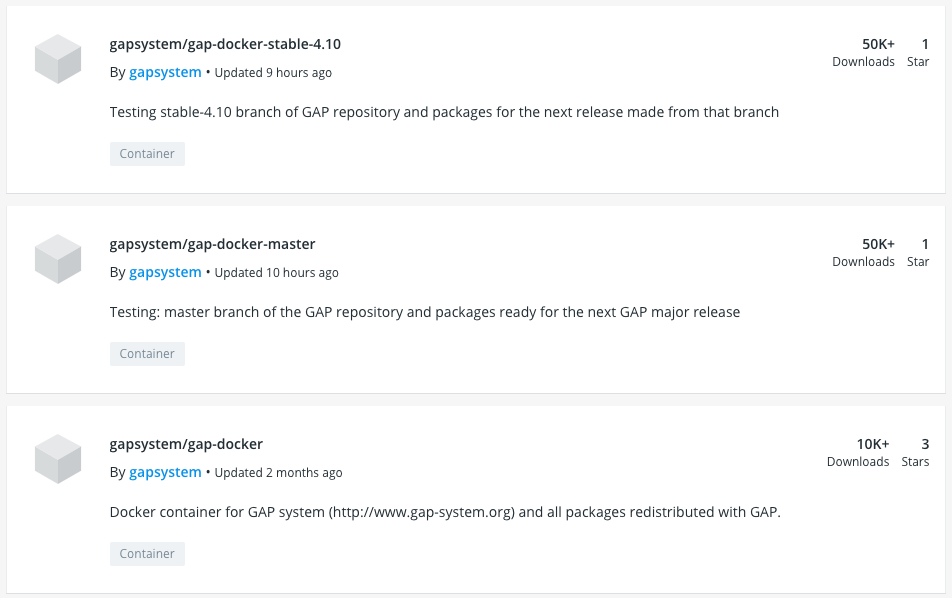
\includegraphics[width=12cm]{images/gap-docker}
    \caption{Selected \GAP Docker containers on Docker Hub}
    \label{fig:gap-docker}
\end{figure}
 
These containers are publicly available on Docker Hub (see Figure~\ref{fig:gap-docker}).
Containers with the development versions of \GAP and packages are updated daily, and have
the largest number of downloads since they are regularly used for testing. An example of
a test using such container could be found under ``Package integration
tests'' in the dashboard shown in 
Figure~\ref{fig:gap-core-tests}. Clicking on the ``status'' button leads to the overview displayed
in Figure~\ref{fig:gap-docker-master-testsuite}, from where one could inspect
test output for each of the configurations. 

\begin{figure}[!ht]
    \centering
    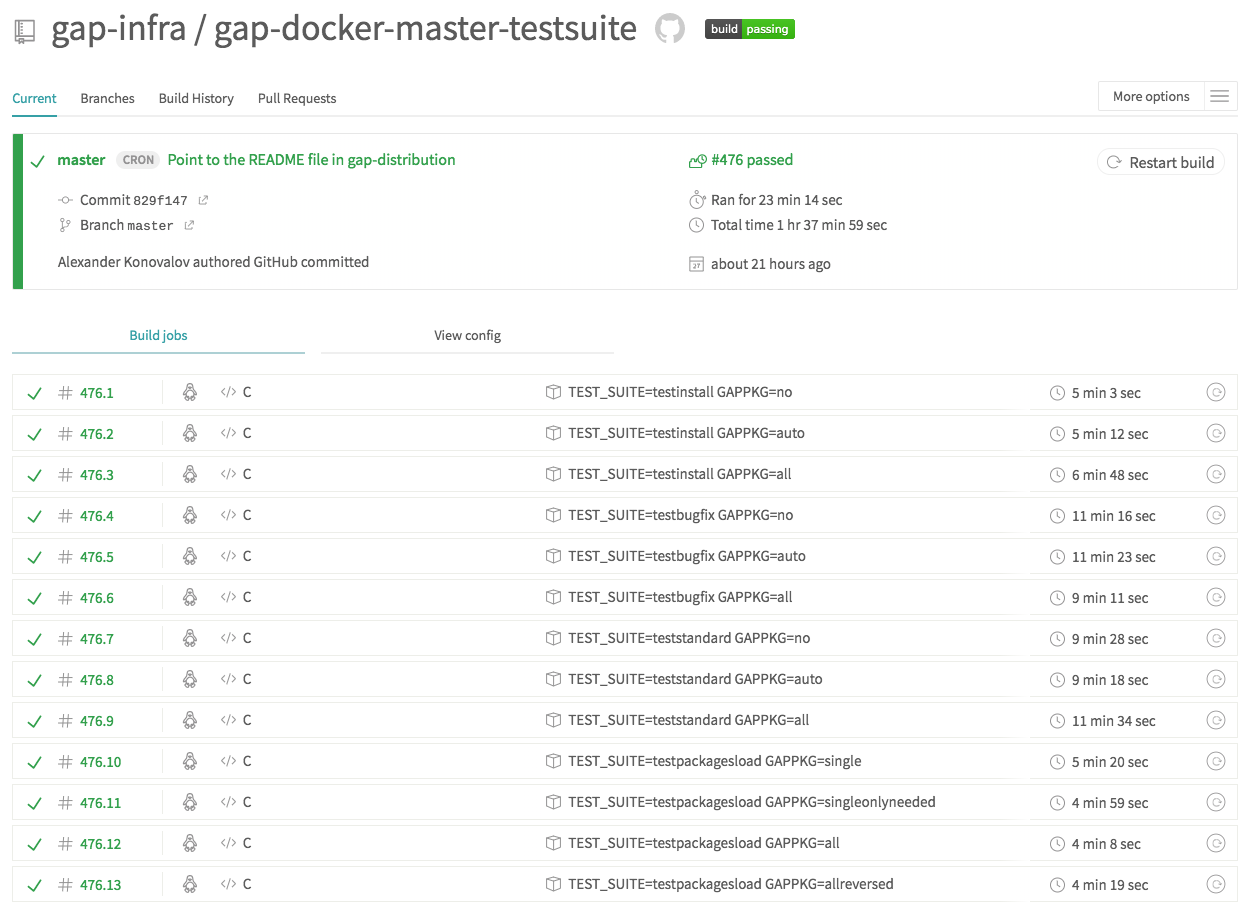
\includegraphics[width=\textwidth]{images/gap-docker-master-testsuite}
    \caption{GAP package integration tests on Travis CI}
    \label{fig:gap-docker-master-testsuite}
\end{figure}

%We made use of \href{https://travis-ci.org/}{Travis CI} and
%\href{https://www.appveyor.com/}{AppVeyor} which are 
%free (for open source projects) continuous integration platforms 
%that can be used to build and test software projects hosted at GitHub.
%\emph{Continuous Integration}, usually abbreviated as {\bf CI} is the process
%automated building and testing for every performed or suggested changes to 
%the source code repository. Using Travis and AppVeyor, one can test changes proposed
%in a pull request \emph{before} they are merged into the main repository.
%At the moment, we use Travis CI for tests on Linux and OS X, and 
%AppVeyor for tests on Windows.

%In addition to that, we started to use \href{https://codecov.io/}{Codecov}
%platform to collect \emph{code coverage} reports for GAP to ensure that our
%regression tests exercise GAP codebase at an acceptable level, and then
%the changes which are submitted via pull request are actually being tested
%by Travis CI. Making these results easily obtainable and publicly available
%had a great effect on the community. Adding new tests to improve code coverage
%is a useful task for new contributors to familiarize themselves with the
%project setup. Making coverage reports available for each pull requests
%facilitates checking code coverage during code review and
%encourages their authors to ensure that their contributions have a good
%quality and their suggested changes are actually being tested. 




%%A crucial role in these developments was played by the enhanced
%%profiling facilities discussed 
%%in Subsection~\ref{gap-4.8}. 
%%GAP~4.8 also introduced the {\tt TestDirectory} function to find
%%(recursively) all {\tt .tst} files from a given directory or a list of 
%%directories and run them using {\tt Test}. Having ability to test
%%changes more efficiently also allowed us to further improve all 
%%tools involved in testing, making their output more informative,
%%and allowing test integration into various automated workflows
%%by a better detection of the test outcomes. 
% the logic seems backwards here. Better test tools let us test better, not v.v.
% What I had in mind was that once we set up the system with the
% state of the testing framework as it was, we were able to "test the testing"
% itself, and improve it - for example, by adding progress indicators,
% report time spent on GC and memory used, etc.




\subsection{Continuous Testing of Package Cross Compatibility Ahead of
\GAP Releases}\label{pkg-update}
For packages redistributed with \GAP, our automatic package update system
checks regularly for new versions on the authors web pages, retrieves them, and then uses them in a
number of checks to ensure that new package releases are compatible with
each other and do not break the functionality of the core \GAP system. The
same process also helps us to check that changes in the core \GAP system
do not break the functionality of the packages redistributed with \GAP.
%% (provided those packages have standard tests that allow us to do that
%% automatically)
This system has dramatically simplified the process of making a \GAP
release or update, for which we need a mutually compatible set of
package versions, also compatible with the new core system. This used
to require extensive negotiation with package authors, and sometimes
took months, even though the number of packages was much smaller. Now
developers have continuous visibility of the functionality and
compatibility of released and upcoming versions of packages and of the
core system, and releases are much faster, delivering new features to
end users without compromising speed of delivery or robustness.

\subsection{Improvements to \GAP Package Tools}\label{sec:package-tools}

Sections \ref{sec:packages} and \ref{meataxe64} among others have shown
that developments important to our goal of a flexible, widely portable high performance
mathematical software system can increasingly occur in packages, as
well as in the core \GAP system. For that reason, as well as pursuit
of the broader goals of \ODK to support a user/developer community, we have attached
considerable priority to a supporting and promoting a healthy \GAP
package ecosystem. We have supported this through the developments
described in subsection~\ref{testing}, together with community
supporting activities described in D2.15, with
good effect. During the \ODK
project we have observed rapid growth of the number of \GAP packages
and of the number of active package
authors as well as steady improvements in the quality of package testing and more frequent
package updates. This has both been supported by, and encouraged, the
development of a wide range of tools to help package authors.

In this section introduce these tools and discuss the
impact which they had on the package ecosystem together with the increased
adoption of the open development model by package authors,

\subsubsection{ReleaseTools and GitHubPagesForGAP}
Our collaborator Max Horn (University of Siegen) developed
{\sf ReleaseTools}\footnote{\url{https://github.com/gap-system/ReleaseTools/}}
and {\sf GitHubPagesForGAP}\footnote{\url{https://github.com/gap-system/GitHubPagesForGAP/}}
which allow package
authors to fully automate the release procedure of a \GAP package hosted on GitHub
and the maintenance of a website for it hosted on GitHub pages,
reducing the time needed to publish it to a matter of minutes.

\subsubsection{The Example Package}
The \GAP package {\sf Example} by Werner Nickel, Greg Gamble and
Alexander Konovalov \cite{example}, which acts as a package template,
has been consistently maintained to track the development of
the packages infrastructure and serves to demonstrate a model use of modern
development tools.
%It switched to using {\tt TestDirectory} to demonstrate how to use 
%multiple test files in a GAP package, and migrated
%to GitHub, using {\sf ReleaseTools/GitHubPagesForGAP}
%for new releases. The guidance for package authors, formerly offered
%as an appendix to the {\sf Example} package manual, was moved to the GAP
%Reference manual in \GAP~4.9 release. Finally, the {\sf Example} package
%demonstrates how to set up Travis CI and CodeCov. Package authors
%may copy its configuration files and adapt them with minimal changes.

\subsubsection{PackageMaker}
To offer an alternative way to create a package,
Max Horn developed a GAP package called
{\sf PackageMaker}\footnote{\url{https://github.com/gap-system/PackageMaker}}
(not yet redistributed with \GAP),
which provides an interactive  ``package wizard''. This allows a
user to fill in the basic details 
of the intended package and then creates all of the files making up
the basic structure of the package. A particularly relevant
strength of this tool is that it hides the additional complexities of
packages which include C or C++ code, removing a barrier to faster implementation
of key kernels.

\subsubsection{AutoDoc}
\GAP packages are required to provide documentation.  The key central
format for \GAP documentation is XML-based, defined in the {\sf
  GAPDoc} package, and while convenient in many ways, can be rather
cumbersome and error prone to write by hand.
In 2012 Sebastian Gutsche 
and Max Horn (both now at the University of Siegen) developed the 
{\sf AutoDoc} package \cite{autodoc} which creates
documentation from simple structured comments in the source code,
similar to pydoc or javadoc.

By now, {\sf AutoDoc} has become very reliable and configurable, and
is in use by 89 GAP packages.
% for building some parts or their whole manuals.
% the number 89 was determined by 
%
% grep 'AutoDoc(' */makedoc.g | wc -l
%
% a note "parts or their whole manuals" is essential - 
% it is possible to build a GAPDoc manual using AutoDoc
% and automatically generate title page, updating the
% metadata from those in PackageInfo.g, avoiding the need
% to duplicate details in two places. The rest of the
% manuals for such packages may still remain in XML.

\subsubsection{Continuous Integration Support for Package Authors}
Using Docker containers described in Section~\ref{sec:gap-infra}
and shown on Figure~\ref{fig:gap-docker} enabled us to make the
results of regression tests for \GAP packages publicly
available via Travis CI. Using a prebuilt docker image 
greatly reduced the runtime of the test and allowed us to
have a separate test configuration for each package,
which is easily discover-able via the Travis CI interface.

Figure~\ref{fig:gap-docker-pkg-tests} shows a fragment of the dashboard
from \url{https://github.com/gap-system/gap-distribution} which 
indicates tests status. In this snapshot, it happens that a package
was depending on undefined behaviour of a \GAP library function, which
was changed, resulting in package tests failing. The prompt detection
of this interaction made it easy to diagnose and 
the author was immediately notified and reacted with a quick
fix. Previously this could have required many weeks of tedious
correspondence to resolve.


% \comment{this must be clear from picture}
%We separate passing and failing tests into different
%Travis jobs, and use that to monitor their status and check that
%changes in GAP do not break package tests. 

\begin{figure}[!ht]
    \centering
    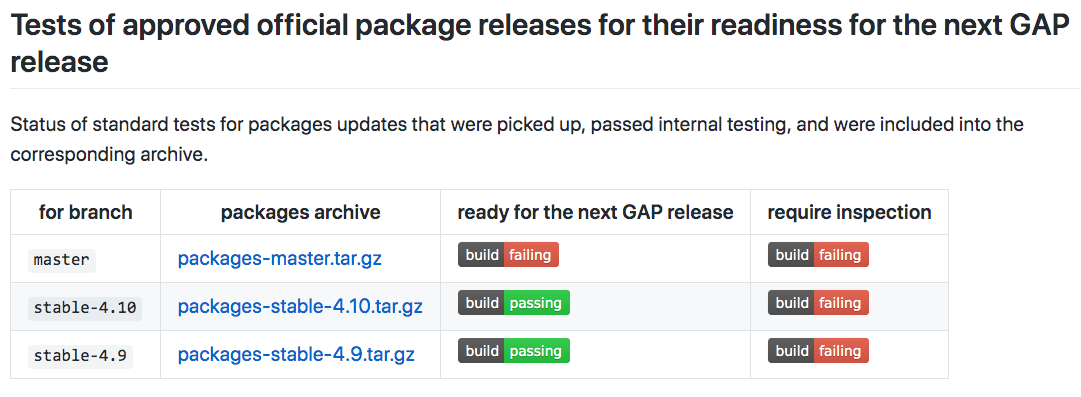
\includegraphics[width=\textwidth]{images/gap-docker-pkg-tests}
    \caption{Dashboard for Travis tests of \GAP packages (GitHub view)}
    \label{fig:gap-docker-pkg-tests}
\end{figure}


%% \comment{not sure if  Figure~\ref{fig:gap-infra-travis} adds anything new
%% - may be deleted?}
%% The setup for such tests is organized in the gap-infra GitHub organisation
%% (\url{https://github.com/gap-infra}. Figure~\ref{fig:gap-infra-travis} shows a 
%% screenshot of a dashboard which indicates tests status.
%% \comment{All these screenshots may be superfluous - I made them to show
%% what could be included, we can remove some or cut parts of them out later}

%% \begin{figure}[!ht]
%%     \centering
%%     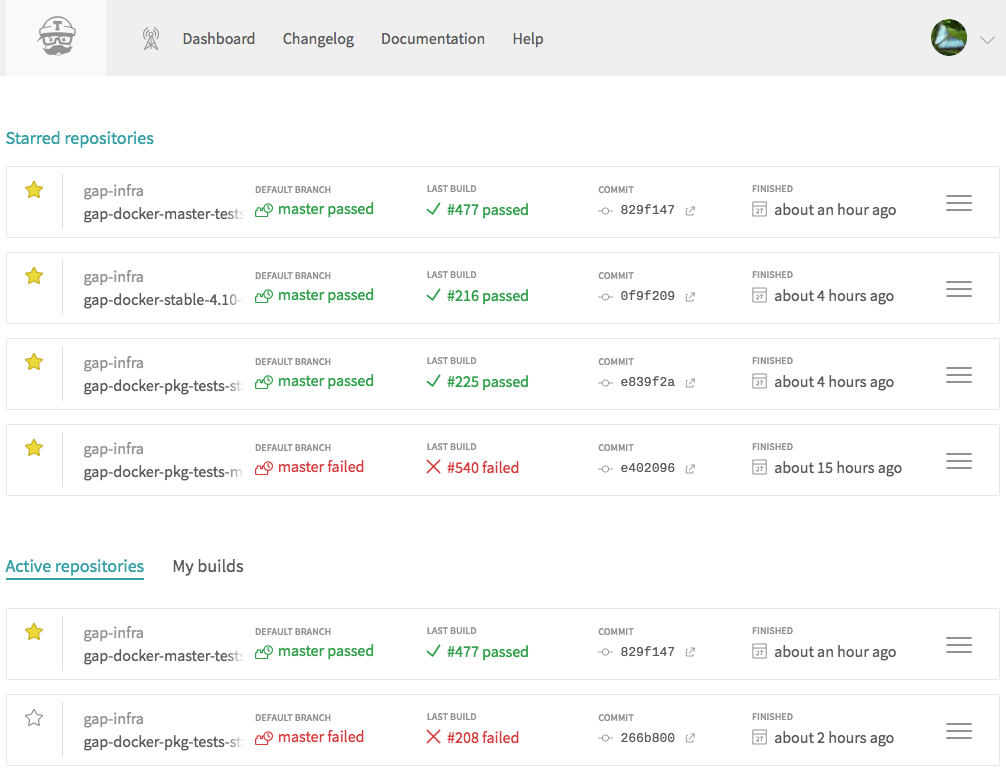
\includegraphics[width=\textwidth]{images/gap-infra-travis}
%%     \caption{Dashboard for Travis tests of \GAP packages (Travis CI view)}
%%     \label{fig:gap-infra-travis}
%% \end{figure}

% \comment{this may be too technical -- no I like it SL}
One of the extensions of the package testing framework, greatly 
facilitated by packages migrating to GitHub, was adding tests not
only for the latest official releases of GAP packages, but also
for their \emph{development} versions.
% https://travis-ci.org/gap-infra/gap-docker-pkg-tests-stable-4.10-devel
% https://travis-ci.org/gap-infra/gap-docker-pkg-tests-master-devel
In this case, the onus to check test outcomes is on package authors,
but they are able to quickly see how the changes that they have made to
a package but not released yet work in different settings (the
released and development versions of \GAP, with various different
combinations of other packages, for instance). Again this leads to
prompt diagnosis and easy fixing of problems, and improves the quality
of released packages.

%% Figure~\ref{fig:gap-packages-travis} shows a screenshot of a 
%% report on the activity in the gap-packages organization 
%% for the last month (for the current version of 
%% this report, check \url{https://travis-ci.org/gap-packages?tab=insights}).

%% \begin{figure}[!ht]
%%     \centering
%%     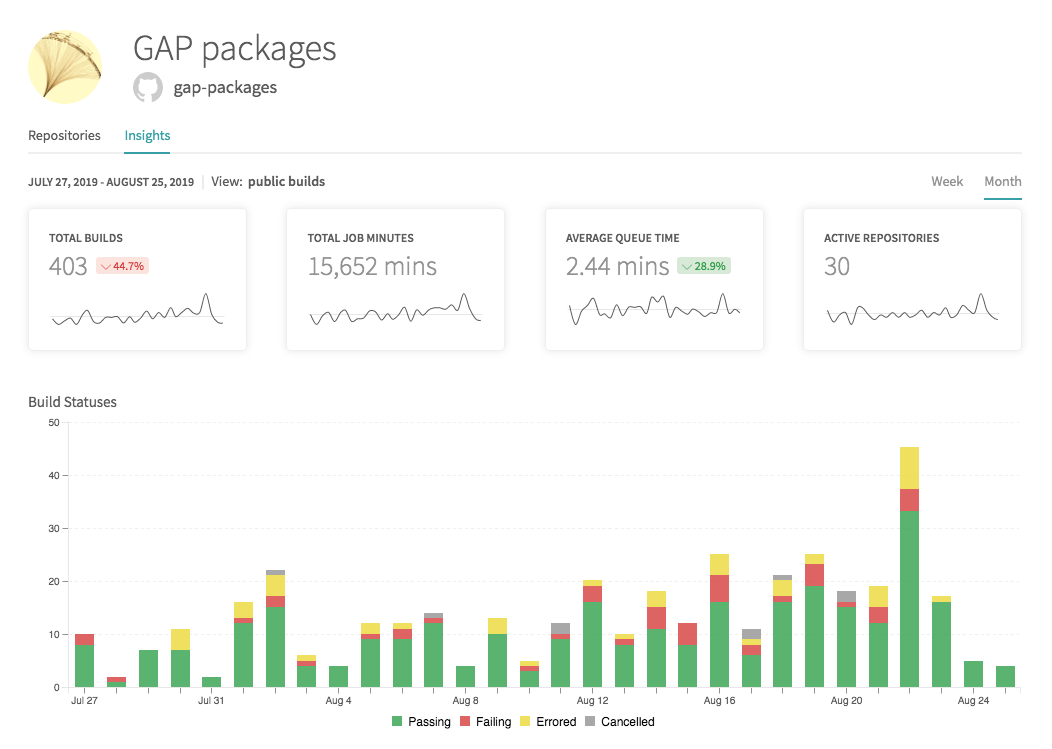
\includegraphics[width=\textwidth]{images/gap-packages-travis}
%%     \caption{Activity of Travis tests in gap-packages GitHub organization}
%%     \label{fig:gap-packages-travis}
%% \end{figure}

Finally, Figure~\ref{fig:gap-packages-codecov} show the code coverage
leaderboard. We aim at ensuring that code coverage for packages is 
not worse than for the core GAP system, but in fact many packages
put a lot of effort in ensuring that their coverage is close to 100\%. 

\begin{figure}[!ht]
    \centering
    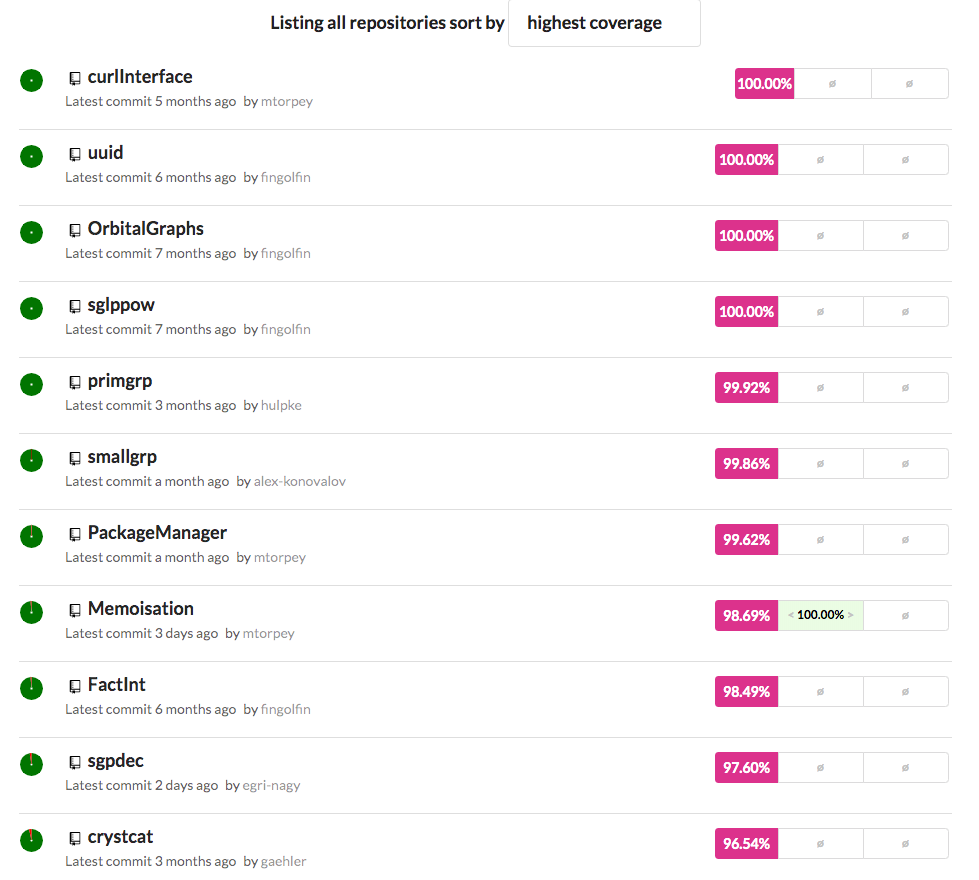
\includegraphics[width=\textwidth]{images/gap-packages-codecov}
    \caption{Codecov leaderboard for in gap-packages GitHub organization}
    \label{fig:gap-packages-codecov}
\end{figure}

\subsection{Open Development of \GAP Packages -- Measure of Uptake
  and Quality}\label{sec:uptake}

As we have explained above, we encourage and support package authors
to use open development models and tools similar to those used for
\GAP itself, since we believe that this is the best way to support the
development of a large portfolio of high quality compatible packages
which meet our users diverse computational requirements.

The openness of our preferred model also provides a number of tools
that we can use to measure our success, both in encouraging uptake and
in some aspects of the quality of the packages.

At the time of writing only 4 packages redistributed with GAP do not
have a public source code repository (to compare, in Month 38 there
were still 23 such packages). In some cases, this required significant
efforts on our part to establish contacts with authors who left
academia, gain their permission and agree a suitable license. We then
had to  populate a repository with a history based on archives of
past releases. In these cases (where we deem the package important
enough,  we formally ``adopt'' the package and declare it to be collectively maintained
by the GAP Group. This work helps ensure that the code will be
preserved in a usable state as \GAP and other tools evolve, something
that is
necessary to check and reproduce computational results. It also gives
visibility to the packages, sometimes attracting new contributors or
even maintainers. As
Figure~\ref{fig:gap-package-tests} shows, the number of individuals
involved in package development increased from 158 in Month 3 to 196
in Month 46.

Figure~\ref{fig:gap-package-releases} shows the number of \GAP packages
included in some \GAP release by year (of the release).
At the beginning of the project, GAP 4.7.9 published in November
2015 included 119 packages, 52\% of which had published a release in 2014--2015.
Now, GAP 4.10.2 includes 145 packages, 88\% of which have published a
release in 2018--2019. The ``long tail'' of packages that haven't been updated for
a long time is gradually reducing, a very encouraging sign of the
vigour of the community.
%(we take measures of not breaking
%existing functionality, but old packages are usually not picking up
%new improvements; and may prevent us from withdrawing obsolete
%functionality).

Larger proportion of recent releases means that 
packages are updated to make use of the recent \GAP developments,
and are responsive to reports about detected problems.
This is greatly facilitated by hosting packages on GitHub making it
easy and convenient for \GAP developers to offer support in the form
of code patches (``pull requests'' in git terminology) or even by
actually publishing releases for them.
%who prefer to overlook mathematical functionality and general development of the
%package but do not want to dive into technicalities of release wrapping.

\begin{figure}[!ht]
    \centering
    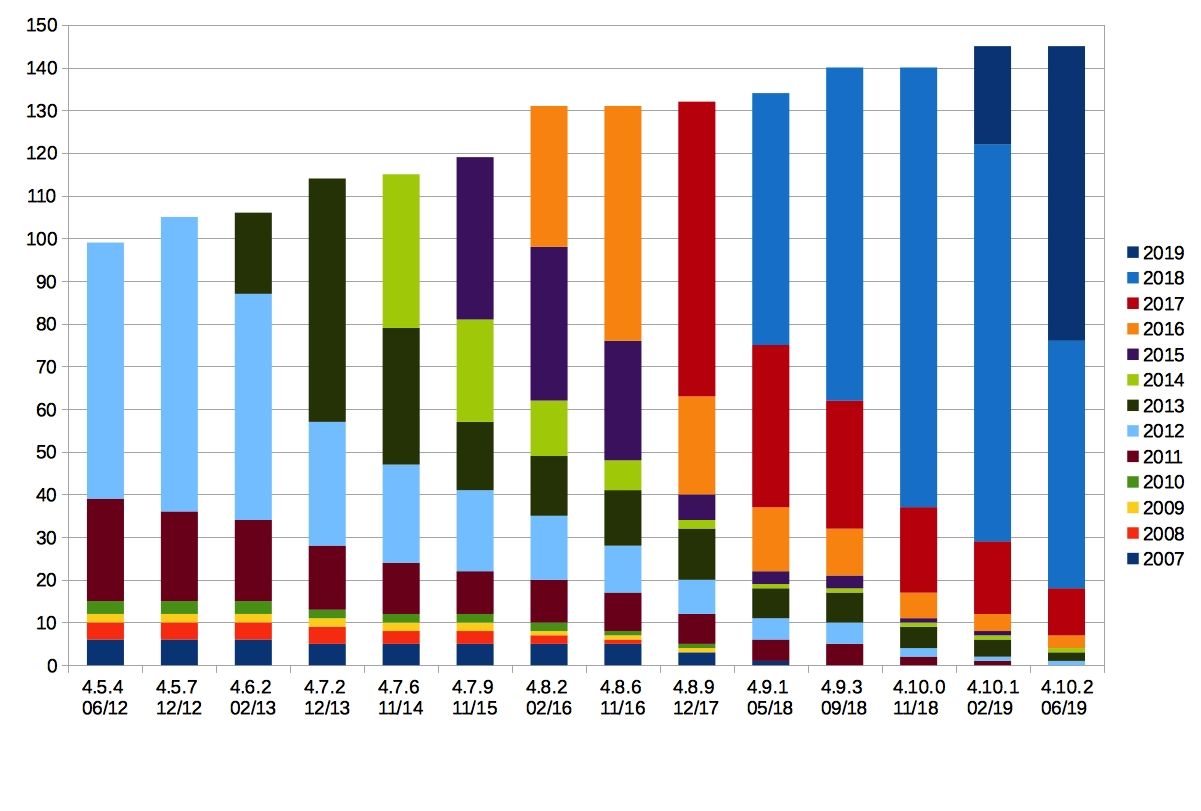
\includegraphics[width=\textwidth]{images/gap-package-releases}
    \caption{Number of \GAP packages and their release year}
    \label{fig:gap-package-releases}
\end{figure}


Over the same period, package releases not only became more frequent,
but their quality also 
improved. In November 2015, 52\% of packages did not provide a standard 
test suite at all, whereas now 78\% of packages have one.
% https://github.com/gap-packages/gap-packages.github.io/issues/9
It is then easy for their authors to  regularly test them 
with published GAP releases and with the development version.
Some have their own continuous integration systems
(e.g. the \href{https://homalg-project.github.io/}{\sf homalg} project,
which uses \href{https://circleci.com/}{CircleCI}).
At the moment of writing, in the stable-4.10 branch,
standard tests pass for 102 packages
% https://travis-ci.org/gap-infra/gap-docker-pkg-tests-stable-4.10
and fail for 12.
% https://travis-ci.org/gap-infra/gap-docker-pkg-tests-stable-4.10-staging 
These failures are probably not serious bugs but variations in output
format, or an incompatibility with some other package
that is not loaded by default).

\begin{figure}[!ht]
    \centering
    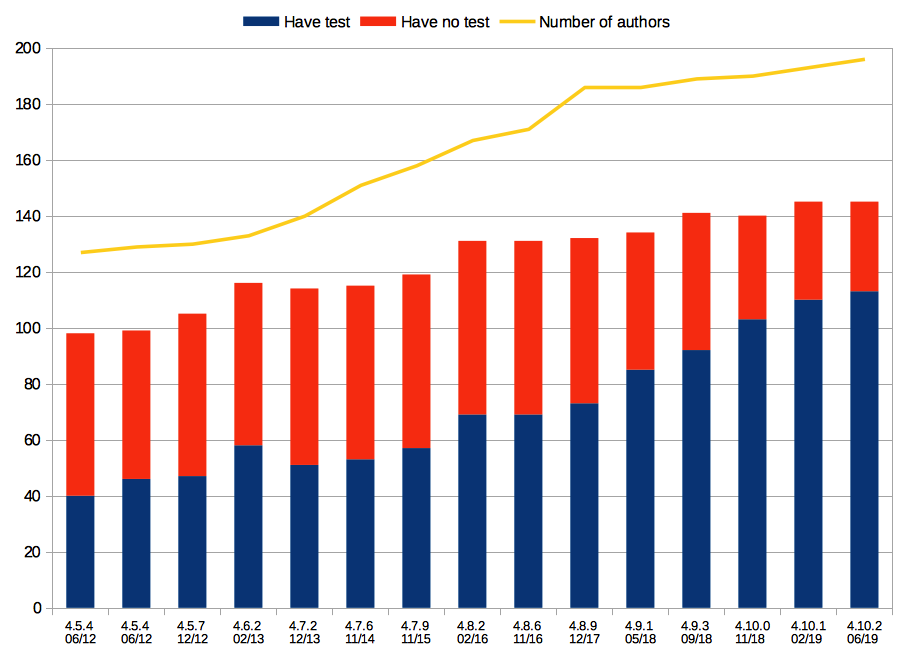
\includegraphics[width=\textwidth]{images/gap-package-tests}
    \caption{Number of \GAP packages, their authors, and packages with tests.}
    \label{fig:gap-package-tests}
\end{figure}

% grep github currentPackageInfoURLList | wc -l
Another illustrative statistics is the number of \GAP packages
whose websites hosted on GitHub pages (some of them use
their own setup, different from {\sf GitHubPagesForGAP}. This is not a
specific suggestion or requirement, but it indicates engagement with
open development  methods, and makes it easy to keep the website up to date.
The following table gives this number for August of each respective year:

\begin{center}
\begin{tabular}{| c | c | c | c | c | c |} 
\hline
Year & 2015 & 2016 & 2017 & 2018 & 2019 \\
\hline
Number of packages & 14 & 45 & 61 & 92 & 124 \\
\hline
\end{tabular}
\end{center}

\subsection{The \GAP package manager}\label{pkg-manager}

\subsubsection{Background}

For many years, the installation of packages in \GAP has been an
entirely manual process.  If a user requires a package that is not
currently installed on their system, they are required to visit the
\GAP website, or the website of the required package, download an
archive or repository and extract it into their package directory.  In
many cases, they must also compile C code or external programs
within the package before use, in a process that is not consistent
between packages.  Worst of all, any packages on which their chosen
package depends must also be installed individually, including all
these steps for each one.

This awkward installation procedure is mitigated by the inclusion of a
large number of packages with the main release archive, which solution
masks the problem for the majority of users, who do not require any
more specialized packages.  However, it also results in a 1.6 GB
standard installation, of which the packages make up 1.4 GB, and while
the files are installed, C code often does not get compiled. While
some packages are used by almost every \GAP user because they enhance
the performance of core \GAP features, only a subset of the others
will be needed by any specific end user. This need may be explicit (when
they load a package relevant to their research interests) or implicit
(to satisfy package dependencies). It would be desirable to avoid all
users having copies of all packages by default.

Additional problems can arise when the \GAP installation is controlled
by central administration and a user needs an extra package installed or a
package compiled, or when a user wishes to update to a new package
version ahead of it being included in a new \GAP distribution.


In the light of these issues, the possibility of a more sophisticated
package management system for \GAP has been discussed for some time,
and was realized with the creation of {\sf PackageManager}
\cite{PackageManager} in Month 37, by Michael Torpey.  Development
started after a discussion at \GAP Days Fall 2018
(\url{https://www.gapdays.de/gapdays2018-fall/}) and an initial
release was made before the end of that meeting.  New features have
been added in various further releases across the past year.

\subsubsection{Design}

{\sf PackageManager} is a \GAP package itself, and is utilized in the
standard way, by loading it into a \GAP session and executing \GAP
functions. This approach to package management was chosen over an external
manager since it allows users to install and remove packages without ever
leaving the \GAP prompt, while making no, or minimal assumptions about
the underlying system setup. This gives
users a comfortable and familiar environment. In most cases, packages can be installed
and loaded without restarting the session, as shown in Figure \ref{fig:pkgman-sample-b}.
This means that users' workflow is interrupted as little as possible, and they do
not need to save and reload their work.

\begin{figure}[!ht]
  \begin{mdframed}
    \centering
    {\tiny
\begin{verbatim}
gap> InstallPackage("digraphs");
#I  Getting PackageInfo URLs...
#I  Retrieving PackageInfo.g from https://gap-packages.github.io/Digraphs/PackageInfo.g ...
#I  Downloading archive from URL https://github.com/gap-packages/Digraphs/releases/download\
/v0.15.4/digraphs-0.15.4.tar.gz ...
#I  Saved archive to /tmp/tmcLM2FI/digraphs-0.15.4.tar.gz
#I  Extracting to /home/user/.gap/pkg/digraphs-0.15.4 ...
#I  Checking dependencies for Digraphs...
#I    io >=4.5.1: true
#I    orb >=4.8.2: true
#I  Running compilation script on /home/user/.gap/pkg/digraphs-0.15.4 ...
true
gap> LoadPackage("digraphs", false);
true
\end{verbatim}
    }
    \end{mdframed}
    \caption{Installing a package using {\sf PackageManager}.}
    \label{fig:pkgman-sample-b}
\end{figure}

The most important function provided by {\sf PackageManager} is
\texttt{InstallPackage}, which can take as argument the URL of an archive, repository, or package info file, or simply the
name of a package.  In the case of a URL, the appropriate file is retrieved
using an internet connection, and used to install the package; if a package name
is given, it is looked up in a pre-defined list of package URLs and installed
from there.  In most cases, the latest released version of a package is
installed, but a user can specify an older version by giving an explicit archive
URL, or a development version by specifying a branch in a
version control repository.
Also provided are \texttt{RemovePackage} and \texttt{UpdatePackage}, which
remove a package or update a package to the latest version, given the package's
name.

The ability to install a package given only its name is useful, but requires
some important design decisions: how do we decide which packages to support, and
which versions do we install by default?  One option would be to have a
centralized repository (as is common for the {\sf APT} package manager) which
contains a carefully checked set of package versions that are known to work with
the installed version of \GAP and with each other; this has the advantage of
stability and control, but may make it harder to get the latest software
versions.  The other option is to store links to appropriate locations on the
package websites, allowing the most recently released version to be installed
without explicit approval from the \GAP authors; this approach is closer to the
more liberal {\sf pip} package manager for the Python language.
In the end, the latter approach was taken for the following reasons:
\begin{itemize}
\item approved package versions for a given release are likely to be included
  with the \GAP installation anyway, and it is unlikely that users would need
  to reinstall these;
\item the latter approach requires no additional infrastructure, since a
  list of URLs for package info files is already maintained for testing purposes;
\item this approach encourages active use, and therefore testing, of recent releases.
\end{itemize}
This decentralized approach has therefore been adopted for the moment, though
future development could move easily towards a different approach.

\subsubsection{Features}

Over the course of {\sf PackageManager}'s development, it has accumulated
various features that automate as much of the installation process as possible.
During installation, the following operations are carried out automatically:
\begin{itemize}
\item any kernel module is configured and compiled, if present;
\item package documentation is built from source if necessary;
\item external software prerequisites are installed using a package-specific
  shell script, if one is present;
\item all missing package dependencies are installed, or recompiled if broken;
\item basic checks are performed to verify that installation was successful.
\end{itemize}

The new packages are installed in a user-specific directory separate
from the \GAP installation, so that multiple users on a shared system
can have distinct package configurations. The packages will also
remain present if the main \GAP installation is moved or replaced.

This has resulted in a reasonably smooth installation process, with very little
friction encountered by a user who tries to get a new package working.
The package manager is
now a deposited package in \GAP, and is therefore distributed in the main
archive with each release.


\subsubsection{Best practice}

{\sf PackageManager} was written using modern open-source software technologies
and practices.  In the report on OpenDreamKit D1.5, in Section 4.3.2, there are
two checklists for best practices: one for software engineering, and one for
dissemination.  The package fulfills all the requirements in both lists, as summarized in
Tables \ref{tab:pkgman-se-check} and \ref{tab:pkgman-diss-check}.

\begin{table}[ht]
  \renewcommand{\arraystretch}{1.2}
  \begin{tabular}{|p{5.1cm}|c|p{9.5cm}|}\hline
    Version control & \checkmark & Git \\ \hline
    Tests & \checkmark & \multirow{2}{*}{\GAP test suite with 99\% code coverage} \\ \cline{1-2}
    Automated tests & \checkmark & \\ \hline
    Continuous integration & \checkmark & Travis runs test suite for every commit \\ \hline
    Automatic building of releases & \checkmark & {\sf ReleaseTools} (see above) \\ \hline
  \end{tabular}
  \vspace{0pt}
  \caption{Software engineering good practice checklist for {\sf PackageManager}}
  \label{tab:pkgman-se-check}
\end{table}

\begin{table}[ht]
  \renewcommand{\arraystretch}{1.2}
  \begin{tabular}{|p{5.1cm}|c|p{9.5cm}|}\hline
    Host code publicly & \checkmark & \url{https://github.com/gap-packages/PackageManager} \\ \hline
    Reference Manual (APIs) & \checkmark & GAPDoc/Autodoc, and hosted on package website \\ \hline
    Tutorial (for beginning users) & \checkmark & \multirow{2}{9.5cm}{Quick examples in readme and manual, before more detailed documentation} \\ \cline{1-2}
    Examples & \checkmark & \\ \hline
    Live interactive online demos & \checkmark & Binder link included in readme \\ \hline
    Support mechanisms & \checkmark & Github issues \\ \hline
    How to cite the output? & \checkmark & Explained on readme and website \\ \hline
    Installation mechanism & \checkmark & Distributed with \GAP, and can update itself \\ \hline
    High level description accessible to non-experts & \checkmark & In readme, and chapter 1 of manual \\ \hline
    URLs/Blog/etc to and from OpenDreamKit project & \checkmark & OpenDreamKit link and logo in readme \\ \hline
    Grant acknowledgments & \checkmark & Acknowledged in readme \\ \hline
    Open Source license & \checkmark & GPL v2 or later \\ \hline
    Workshop & \checkmark & \multirow{2}{9.6cm}{Demos in \textit{CIRCA Seminar} (USTAN, Month 43) and \textit{Workshop on Mathematical Data} (Cernay, Month 48)} \\ \cline{1-2}
    Engaging users & \checkmark & \\ \hline
  \end{tabular}
  \vspace{0pt}
  \caption{Dissemination good practice checklist for {\sf PackageManager}}
  \label{tab:pkgman-diss-check}
\end{table}

\subsubsection{Other uses}

Aside from making the on-demand installation of individual packages easier, {\sf
  PackageManager} has implications for the future of how \GAP is distributed.
There are no current plans to stop distributing
deposited packages with the \GAP archive by default, but the
possibility of distribute a much smaller archive, containing only a few
fundamental packages and {\sf
  PackageManager} itself and then installing others as needed is now
opened up.  Furthermore, the package manager
can be used by other systems that interact with \GAP to manage
their \GAP installations more easily.  The \cocalc system now contains {\sf PackageManager}
as part of its \GAP 4.10.2 installation, enabling each user to install any
packages they need without \cocalc operators being forced to manage these
installations separately.  This is an example of positive two-way interaction
with \cocalc, and sets as a good precedent for interaction with other
systems.




\subsection{Improvements to \GAP Package Tools}\label{sec:package-tools}

Sections \ref{sec:packages} and \ref{meataxe64} among others have shown
that developments important to our goal of a flexible, widely portable high performance
mathematical software system can increasingly occur in packages, as
well as in the core \GAP system. For that reason, as well as pursuit
of the broader goals of \ODK to support a user/developer community, we have attached
considerable priority to a supporting and promoting a healthy \GAP
package ecosystem. We have supported this through the developments
described in subsection~\ref{testing}, together with community
supporting activities described in D2.15, with
good effect. During the \ODK
project we have observed rapid growth of the number of \GAP packages
and of the number of active package
authors as well as steady improvements in the quality of package testing and more frequent
package updates. This has both been supported by, and encouraged, the
development of a wide range of tools to help package authors.

In this section introduce these tools and discuss the
impact which they had on the package ecosystem together with the increased
adoption of the open development model by package authors,

\subsubsection{ReleaseTools and GitHubPagesForGAP}
Our collaborator Max Horn (University of Siegen) developed
{\sf ReleaseTools}\footnote{\url{https://github.com/gap-system/ReleaseTools/}}
and {\sf GitHubPagesForGAP}\footnote{\url{https://github.com/gap-system/GitHubPagesForGAP/}}
which allow package
authors to fully automate the release procedure of a \GAP package hosted on GitHub
and the maintenance of a website for it hosted on GitHub pages,
reducing the time needed to publish it to a matter of minutes.

\subsubsection{The Example Package}
The \GAP package {\sf Example} by Werner Nickel, Greg Gamble and
Alexander Konovalov \cite{example}, which acts as a package template,
has been consistently maintained to track the development of
the packages infrastructure and serves to demonstrate a model use of modern
development tools.
%It switched to using {\tt TestDirectory} to demonstrate how to use 
%multiple test files in a GAP package, and migrated
%to GitHub, using {\sf ReleaseTools/GitHubPagesForGAP}
%for new releases. The guidance for package authors, formerly offered
%as an appendix to the {\sf Example} package manual, was moved to the GAP
%Reference manual in \GAP~4.9 release. Finally, the {\sf Example} package
%demonstrates how to set up Travis CI and CodeCov. Package authors
%may copy its configuration files and adapt them with minimal changes.

\subsubsection{PackageMaker}
To offer an alternative way to create a package,
Max Horn developed a GAP package called
{\sf PackageMaker}\footnote{\url{https://github.com/gap-system/PackageMaker}}
(not yet redistributed with \GAP),
which provides an interactive  ``package wizard''. This allows a
user to fill in the basic details 
of the intended package and then creates all of the files making up
the basic structure of the package. A particularly relevant
strength of this tool is that it hides the additional complexities of
packages which include C or C++ code, removing a barrier to faster implementation
of key kernels.

\subsubsection{AutoDoc}
\GAP packages are required to provide documentation.  The key central
format for \GAP documentation is XML-based, defined in the {\sf
  GAPDoc} package, and while convenient in many ways, can be rather
cumbersome and error prone to write by hand.
In 2012 Sebastian Gutsche 
and Max Horn (both now at the University of Siegen) developed the 
{\sf AutoDoc} package \cite{autodoc} which creates
documentation from simple structured comments in the source code,
similar to pydoc or javadoc.

By now, {\sf AutoDoc} has become very reliable and configurable, and
is in use by 89 GAP packages.
% for building some parts or their whole manuals.
% the number 89 was determined by 
%
% grep 'AutoDoc(' */makedoc.g | wc -l
%
% a note "parts or their whole manuals" is essential - 
% it is possible to build a GAPDoc manual using AutoDoc
% and automatically generate title page, updating the
% metadata from those in PackageInfo.g, avoiding the need
% to duplicate details in two places. The rest of the
% manuals for such packages may still remain in XML.

\subsubsection{Continuous Integration Support for Package Authors}
Using Docker containers described in Section~\ref{sec:gap-infra}
and shown on Figure~\ref{fig:gap-docker} enabled us to make the
results of regression tests for \GAP packages publicly
available via Travis CI. Using a prebuilt docker image 
greatly reduced the runtime of the test and allowed us to
have a separate test configuration for each package,
which is easily discover-able via the Travis CI interface.

Figure~\ref{fig:gap-docker-pkg-tests} shows a fragment of the dashboard
from \url{https://github.com/gap-system/gap-distribution} which 
indicates tests status. In this snapshot, it happens that a package
was depending on undefined behaviour of a \GAP library function, which
was changed, resulting in package tests failing. The prompt detection
of this interaction made it easy to diagnose and 
the author was immediately notified and reacted with a quick
fix. Previously this could have required many weeks of tedious
correspondence to resolve.


% \comment{this must be clear from picture}
%We separate passing and failing tests into different
%Travis jobs, and use that to monitor their status and check that
%changes in GAP do not break package tests. 

\begin{figure}[!ht]
    \centering
    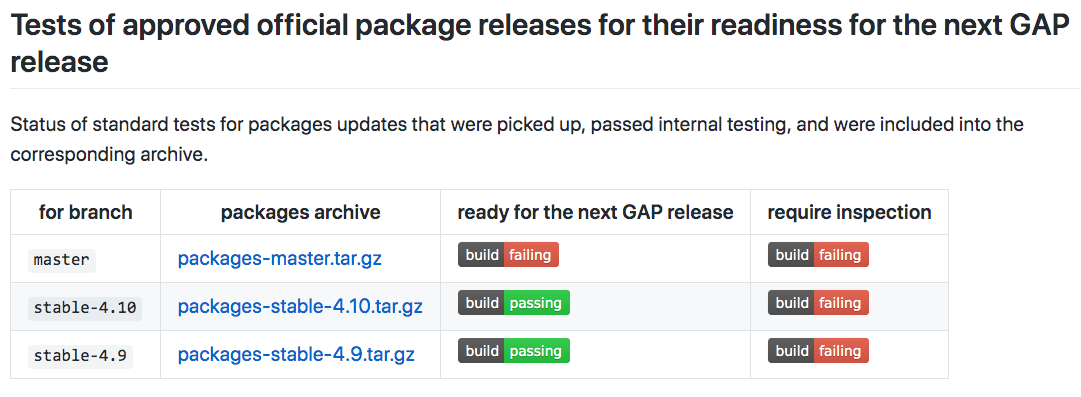
\includegraphics[width=\textwidth]{images/gap-docker-pkg-tests}
    \caption{Dashboard for Travis tests of \GAP packages (GitHub view)}
    \label{fig:gap-docker-pkg-tests}
\end{figure}


%% \comment{not sure if  Figure~\ref{fig:gap-infra-travis} adds anything new
%% - may be deleted?}
%% The setup for such tests is organized in the gap-infra GitHub organisation
%% (\url{https://github.com/gap-infra}. Figure~\ref{fig:gap-infra-travis} shows a 
%% screenshot of a dashboard which indicates tests status.
%% \comment{All these screenshots may be superfluous - I made them to show
%% what could be included, we can remove some or cut parts of them out later}

%% \begin{figure}[!ht]
%%     \centering
%%     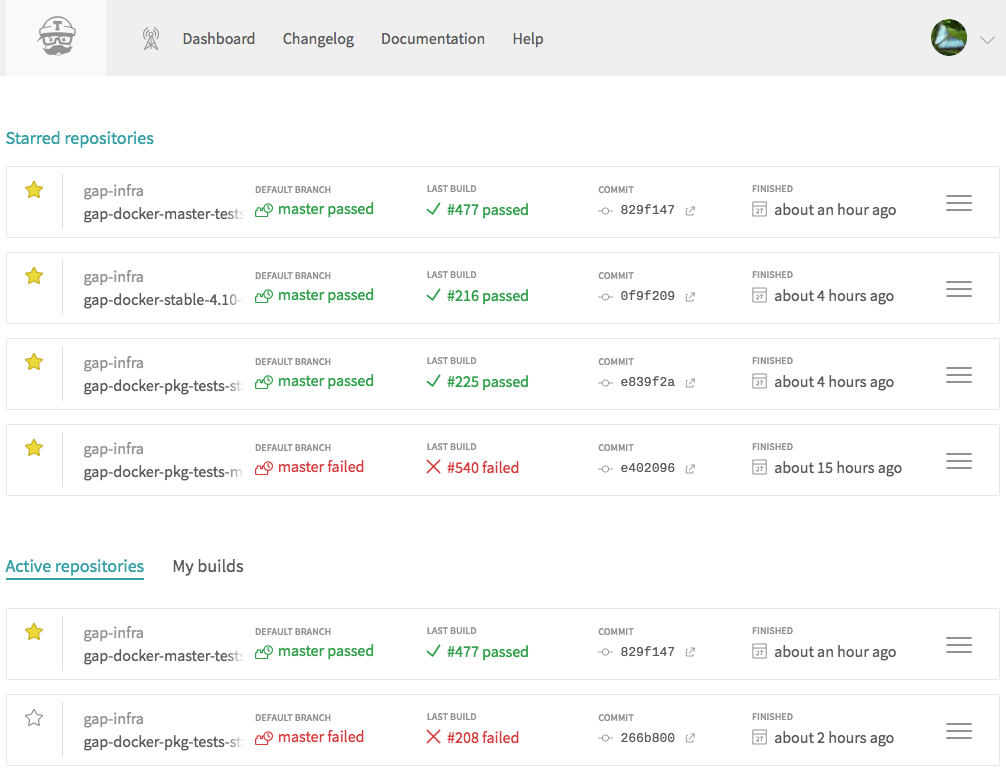
\includegraphics[width=\textwidth]{images/gap-infra-travis}
%%     \caption{Dashboard for Travis tests of \GAP packages (Travis CI view)}
%%     \label{fig:gap-infra-travis}
%% \end{figure}

% \comment{this may be too technical -- no I like it SL}
One of the extensions of the package testing framework, greatly 
facilitated by packages migrating to GitHub, was adding tests not
only for the latest official releases of GAP packages, but also
for their \emph{development} versions.
% https://travis-ci.org/gap-infra/gap-docker-pkg-tests-stable-4.10-devel
% https://travis-ci.org/gap-infra/gap-docker-pkg-tests-master-devel
In this case, the onus to check test outcomes is on package authors,
but they are able to quickly see how the changes that they have made to
a package but not released yet work in different settings (the
released and development versions of \GAP, with various different
combinations of other packages, for instance). Again this leads to
prompt diagnosis and easy fixing of problems, and improves the quality
of released packages.

%% Figure~\ref{fig:gap-packages-travis} shows a screenshot of a 
%% report on the activity in the gap-packages organization 
%% for the last month (for the current version of 
%% this report, check \url{https://travis-ci.org/gap-packages?tab=insights}).

%% \begin{figure}[!ht]
%%     \centering
%%     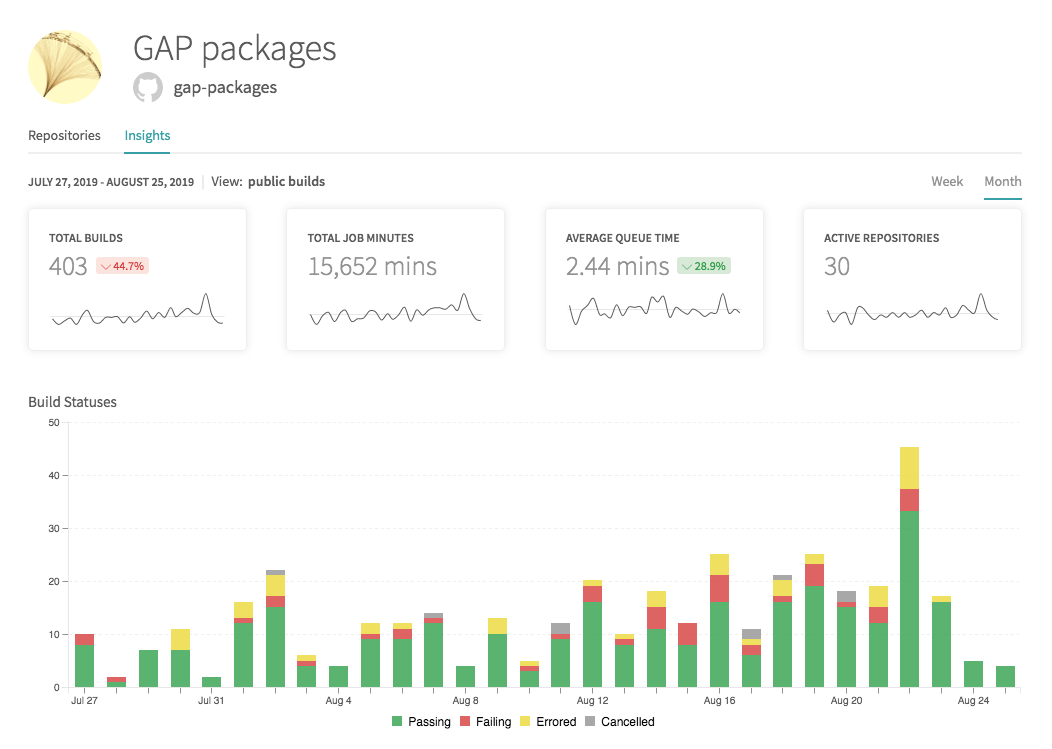
\includegraphics[width=\textwidth]{images/gap-packages-travis}
%%     \caption{Activity of Travis tests in gap-packages GitHub organization}
%%     \label{fig:gap-packages-travis}
%% \end{figure}

Finally, Figure~\ref{fig:gap-packages-codecov} show the code coverage
leaderboard. We aim at ensuring that code coverage for packages is 
not worse than for the core GAP system, but in fact many packages
put a lot of effort in ensuring that their coverage is close to 100\%. 

\begin{figure}[!ht]
    \centering
    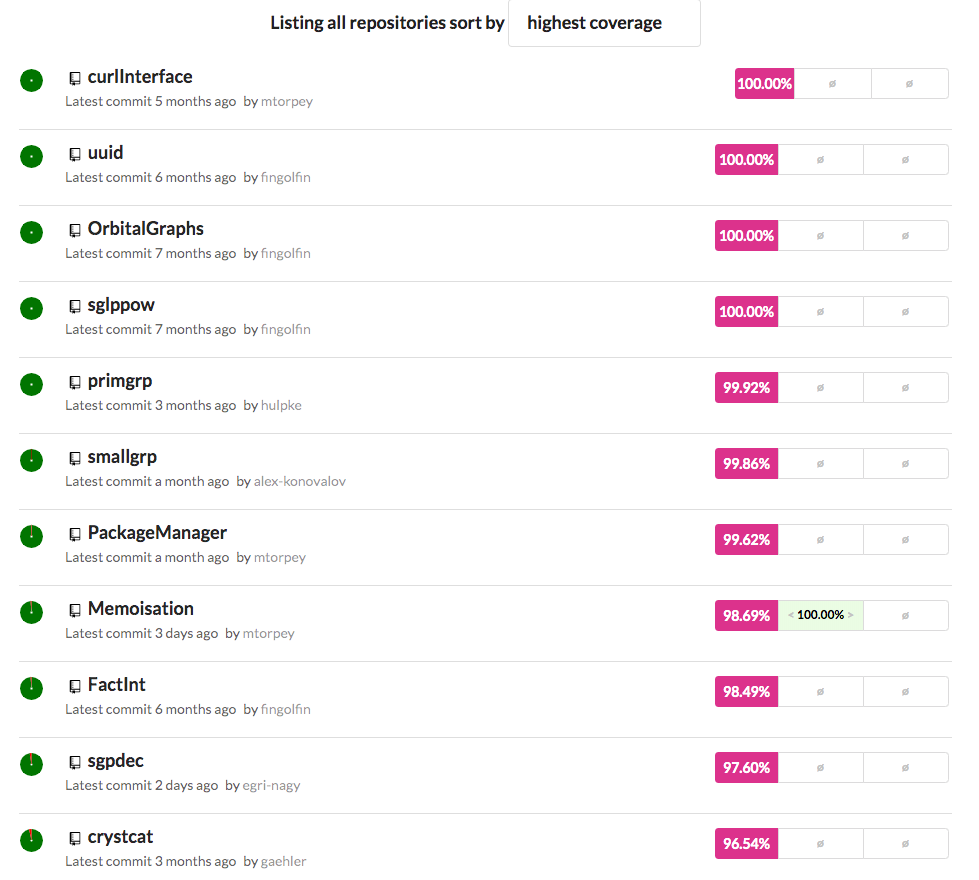
\includegraphics[width=\textwidth]{images/gap-packages-codecov}
    \caption{Codecov leaderboard for in gap-packages GitHub organization}
    \label{fig:gap-packages-codecov}
\end{figure}

\subsection{Open Development of \GAP Packages -- Measure of Uptake
  and Quality}\label{sec:uptake}

As we have explained above, we encourage and support package authors
to use open development models and tools similar to those used for
\GAP itself, since we believe that this is the best way to support the
development of a large portfolio of high quality compatible packages
which meet our users diverse computational requirements.

The openness of our preferred model also provides a number of tools
that we can use to measure our success, both in encouraging uptake and
in some aspects of the quality of the packages.

At the time of writing only 4 packages redistributed with GAP do not
have a public source code repository (to compare, in Month 38 there
were still 23 such packages). In some cases, this required significant
efforts on our part to establish contacts with authors who left
academia, gain their permission and agree a suitable license. We then
had to  populate a repository with a history based on archives of
past releases. In these cases (where we deem the package important
enough,  we formally ``adopt'' the package and declare it to be collectively maintained
by the GAP Group. This work helps ensure that the code will be
preserved in a usable state as \GAP and other tools evolve, something
that is
necessary to check and reproduce computational results. It also gives
visibility to the packages, sometimes attracting new contributors or
even maintainers. As
Figure~\ref{fig:gap-package-tests} shows, the number of individuals
involved in package development increased from 158 in Month 3 to 196
in Month 46.

Figure~\ref{fig:gap-package-releases} shows the number of \GAP packages
included in some \GAP release by year (of the release).
At the beginning of the project, GAP 4.7.9 published in November
2015 included 119 packages, 52\% of which had published a release in 2014--2015.
Now, GAP 4.10.2 includes 145 packages, 88\% of which have published a
release in 2018--2019. The ``long tail'' of packages that haven't been updated for
a long time is gradually reducing, a very encouraging sign of the
vigour of the community.
%(we take measures of not breaking
%existing functionality, but old packages are usually not picking up
%new improvements; and may prevent us from withdrawing obsolete
%functionality).

Larger proportion of recent releases means that 
packages are updated to make use of the recent \GAP developments,
and are responsive to reports about detected problems.
This is greatly facilitated by hosting packages on GitHub making it
easy and convenient for \GAP developers to offer support in the form
of code patches (``pull requests'' in git terminology) or even by
actually publishing releases for them.
%who prefer to overlook mathematical functionality and general development of the
%package but do not want to dive into technicalities of release wrapping.

\begin{figure}[!ht]
    \centering
    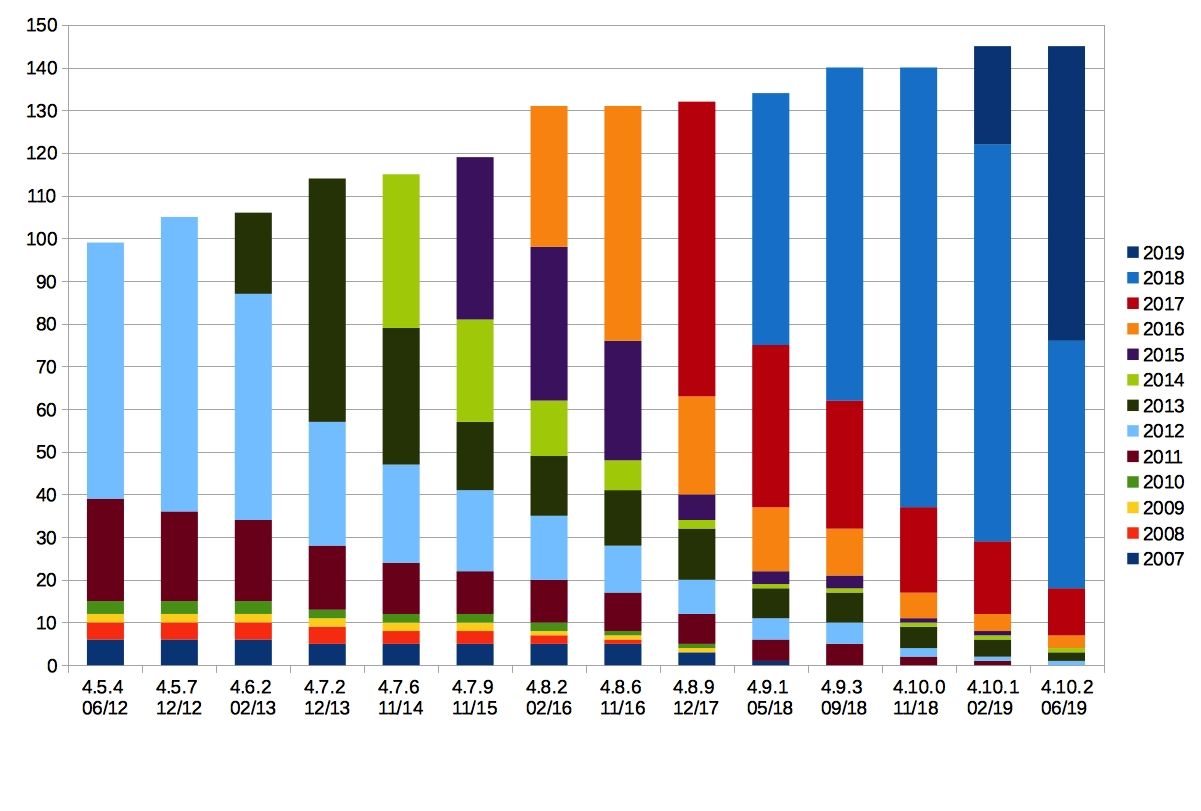
\includegraphics[width=\textwidth]{images/gap-package-releases}
    \caption{Number of \GAP packages and their release year}
    \label{fig:gap-package-releases}
\end{figure}


Over the same period, package releases not only became more frequent,
but their quality also 
improved. In November 2015, 52\% of packages did not provide a standard 
test suite at all, whereas now 78\% of packages have one.
% https://github.com/gap-packages/gap-packages.github.io/issues/9
It is then easy for their authors to  regularly test them 
with published GAP releases and with the development version.
Some have their own continuous integration systems
(e.g. the \href{https://homalg-project.github.io/}{\sf homalg} project,
which uses \href{https://circleci.com/}{CircleCI}).
At the moment of writing, in the stable-4.10 branch,
standard tests pass for 102 packages
% https://travis-ci.org/gap-infra/gap-docker-pkg-tests-stable-4.10
and fail for 12.
% https://travis-ci.org/gap-infra/gap-docker-pkg-tests-stable-4.10-staging 
These failures are probably not serious bugs but variations in output
format, or an incompatibility with some other package
that is not loaded by default).

\begin{figure}[!ht]
    \centering
    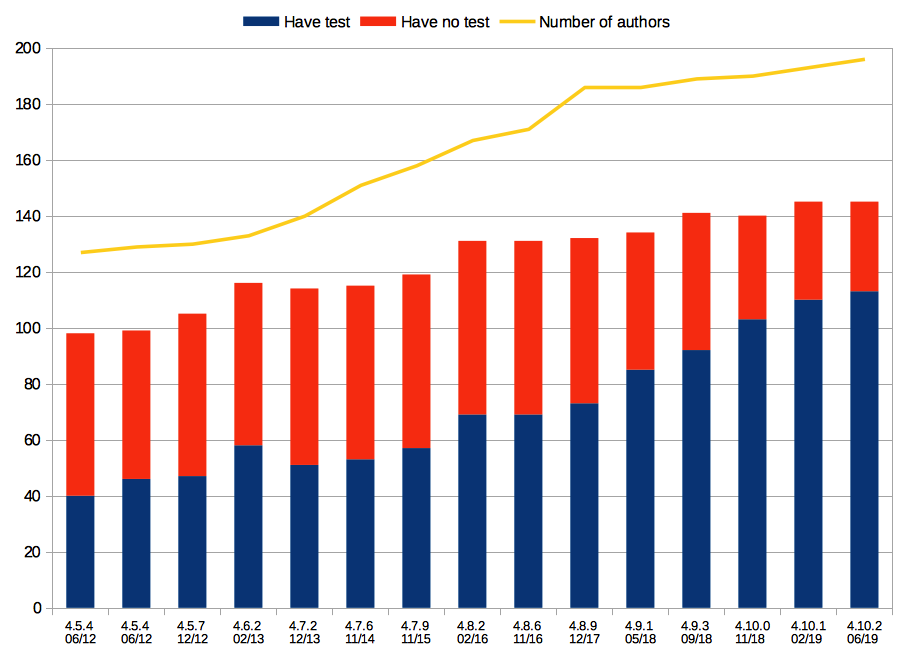
\includegraphics[width=\textwidth]{images/gap-package-tests}
    \caption{Number of \GAP packages, their authors, and packages with tests.}
    \label{fig:gap-package-tests}
\end{figure}

% grep github currentPackageInfoURLList | wc -l
Another illustrative statistics is the number of \GAP packages
whose websites hosted on GitHub pages (some of them use
their own setup, different from {\sf GitHubPagesForGAP}. This is not a
specific suggestion or requirement, but it indicates engagement with
open development  methods, and makes it easy to keep the website up to date.
The following table gives this number for August of each respective year:

\begin{center}
\begin{tabular}{| c | c | c | c | c | c |} 
\hline
Year & 2015 & 2016 & 2017 & 2018 & 2019 \\
\hline
Number of packages & 14 & 45 & 61 & 92 & 124 \\
\hline
\end{tabular}
\end{center}

\subsection{The \GAP package manager}\label{pkg-manager}

\subsubsection{Background}

For many years, the installation of packages in \GAP has been an
entirely manual process.  If a user requires a package that is not
currently installed on their system, they are required to visit the
\GAP website, or the website of the required package, download an
archive or repository and extract it into their package directory.  In
many cases, they must also compile C code or external programs
within the package before use, in a process that is not consistent
between packages.  Worst of all, any packages on which their chosen
package depends must also be installed individually, including all
these steps for each one.

This awkward installation procedure is mitigated by the inclusion of a
large number of packages with the main release archive, which solution
masks the problem for the majority of users, who do not require any
more specialized packages.  However, it also results in a 1.6 GB
standard installation, of which the packages make up 1.4 GB, and while
the files are installed, C code often does not get compiled. While
some packages are used by almost every \GAP user because they enhance
the performance of core \GAP features, only a subset of the others
will be needed by any specific end user. This need may be explicit (when
they load a package relevant to their research interests) or implicit
(to satisfy package dependencies). It would be desirable to avoid all
users having copies of all packages by default.

Additional problems can arise when the \GAP installation is controlled
by central administration and a user needs an extra package installed or a
package compiled, or when a user wishes to update to a new package
version ahead of it being included in a new \GAP distribution.


In the light of these issues, the possibility of a more sophisticated
package management system for \GAP has been discussed for some time,
and was realized with the creation of {\sf PackageManager}
\cite{PackageManager} in Month 37, by Michael Torpey.  Development
started after a discussion at \GAP Days Fall 2018
(\url{https://www.gapdays.de/gapdays2018-fall/}) and an initial
release was made before the end of that meeting.  New features have
been added in various further releases across the past year.

\subsubsection{Design}

{\sf PackageManager} is a \GAP package itself, and is utilized in the
standard way, by loading it into a \GAP session and executing \GAP
functions. This approach to package management was chosen over an external
manager since it allows users to install and remove packages without ever
leaving the \GAP prompt, while making no, or minimal assumptions about
the underlying system setup. This gives
users a comfortable and familiar environment. In most cases, packages can be installed
and loaded without restarting the session, as shown in Figure \ref{fig:pkgman-sample-b}.
This means that users' workflow is interrupted as little as possible, and they do
not need to save and reload their work.

\begin{figure}[!ht]
  \begin{mdframed}
    \centering
    {\tiny
\begin{verbatim}
gap> InstallPackage("digraphs");
#I  Getting PackageInfo URLs...
#I  Retrieving PackageInfo.g from https://gap-packages.github.io/Digraphs/PackageInfo.g ...
#I  Downloading archive from URL https://github.com/gap-packages/Digraphs/releases/download\
/v0.15.4/digraphs-0.15.4.tar.gz ...
#I  Saved archive to /tmp/tmcLM2FI/digraphs-0.15.4.tar.gz
#I  Extracting to /home/user/.gap/pkg/digraphs-0.15.4 ...
#I  Checking dependencies for Digraphs...
#I    io >=4.5.1: true
#I    orb >=4.8.2: true
#I  Running compilation script on /home/user/.gap/pkg/digraphs-0.15.4 ...
true
gap> LoadPackage("digraphs", false);
true
\end{verbatim}
    }
    \end{mdframed}
    \caption{Installing a package using {\sf PackageManager}.}
    \label{fig:pkgman-sample-b}
\end{figure}

The most important function provided by {\sf PackageManager} is
\texttt{InstallPackage}, which can take as argument the URL of an archive, repository, or package info file, or simply the
name of a package.  In the case of a URL, the appropriate file is retrieved
using an internet connection, and used to install the package; if a package name
is given, it is looked up in a pre-defined list of package URLs and installed
from there.  In most cases, the latest released version of a package is
installed, but a user can specify an older version by giving an explicit archive
URL, or a development version by specifying a branch in a
version control repository.
Also provided are \texttt{RemovePackage} and \texttt{UpdatePackage}, which
remove a package or update a package to the latest version, given the package's
name.

The ability to install a package given only its name is useful, but requires
some important design decisions: how do we decide which packages to support, and
which versions do we install by default?  One option would be to have a
centralized repository (as is common for the {\sf APT} package manager) which
contains a carefully checked set of package versions that are known to work with
the installed version of \GAP and with each other; this has the advantage of
stability and control, but may make it harder to get the latest software
versions.  The other option is to store links to appropriate locations on the
package websites, allowing the most recently released version to be installed
without explicit approval from the \GAP authors; this approach is closer to the
more liberal {\sf pip} package manager for the Python language.
In the end, the latter approach was taken for the following reasons:
\begin{itemize}
\item approved package versions for a given release are likely to be included
  with the \GAP installation anyway, and it is unlikely that users would need
  to reinstall these;
\item the latter approach requires no additional infrastructure, since a
  list of URLs for package info files is already maintained for testing purposes;
\item this approach encourages active use, and therefore testing, of recent releases.
\end{itemize}
This decentralized approach has therefore been adopted for the moment, though
future development could move easily towards a different approach.

\subsubsection{Features}

Over the course of {\sf PackageManager}'s development, it has accumulated
various features that automate as much of the installation process as possible.
During installation, the following operations are carried out automatically:
\begin{itemize}
\item any kernel module is configured and compiled, if present;
\item package documentation is built from source if necessary;
\item external software prerequisites are installed using a package-specific
  shell script, if one is present;
\item all missing package dependencies are installed, or recompiled if broken;
\item basic checks are performed to verify that installation was successful.
\end{itemize}

The new packages are installed in a user-specific directory separate
from the \GAP installation, so that multiple users on a shared system
can have distinct package configurations. The packages will also
remain present if the main \GAP installation is moved or replaced.

This has resulted in a reasonably smooth installation process, with very little
friction encountered by a user who tries to get a new package working.
The package manager is
now a deposited package in \GAP, and is therefore distributed in the main
archive with each release.


\subsubsection{Best practice}

{\sf PackageManager} was written using modern open-source software technologies
and practices.  In the report on OpenDreamKit D1.5, in Section 4.3.2, there are
two checklists for best practices: one for software engineering, and one for
dissemination.  The package fulfills all the requirements in both lists, as summarized in
Tables \ref{tab:pkgman-se-check} and \ref{tab:pkgman-diss-check}.

\begin{table}[ht]
  \renewcommand{\arraystretch}{1.2}
  \begin{tabular}{|p{5.1cm}|c|p{9.5cm}|}\hline
    Version control & \checkmark & Git \\ \hline
    Tests & \checkmark & \multirow{2}{*}{\GAP test suite with 99\% code coverage} \\ \cline{1-2}
    Automated tests & \checkmark & \\ \hline
    Continuous integration & \checkmark & Travis runs test suite for every commit \\ \hline
    Automatic building of releases & \checkmark & {\sf ReleaseTools} (see above) \\ \hline
  \end{tabular}
  \vspace{0pt}
  \caption{Software engineering good practice checklist for {\sf PackageManager}}
  \label{tab:pkgman-se-check}
\end{table}

\begin{table}[ht]
  \renewcommand{\arraystretch}{1.2}
  \begin{tabular}{|p{5.1cm}|c|p{9.5cm}|}\hline
    Host code publicly & \checkmark & \url{https://github.com/gap-packages/PackageManager} \\ \hline
    Reference Manual (APIs) & \checkmark & GAPDoc/Autodoc, and hosted on package website \\ \hline
    Tutorial (for beginning users) & \checkmark & \multirow{2}{9.5cm}{Quick examples in readme and manual, before more detailed documentation} \\ \cline{1-2}
    Examples & \checkmark & \\ \hline
    Live interactive online demos & \checkmark & Binder link included in readme \\ \hline
    Support mechanisms & \checkmark & Github issues \\ \hline
    How to cite the output? & \checkmark & Explained on readme and website \\ \hline
    Installation mechanism & \checkmark & Distributed with \GAP, and can update itself \\ \hline
    High level description accessible to non-experts & \checkmark & In readme, and chapter 1 of manual \\ \hline
    URLs/Blog/etc to and from OpenDreamKit project & \checkmark & OpenDreamKit link and logo in readme \\ \hline
    Grant acknowledgments & \checkmark & Acknowledged in readme \\ \hline
    Open Source license & \checkmark & GPL v2 or later \\ \hline
    Workshop & \checkmark & \multirow{2}{9.6cm}{Demos in \textit{CIRCA Seminar} (USTAN, Month 43) and \textit{Workshop on Mathematical Data} (Cernay, Month 48)} \\ \cline{1-2}
    Engaging users & \checkmark & \\ \hline
  \end{tabular}
  \vspace{0pt}
  \caption{Dissemination good practice checklist for {\sf PackageManager}}
  \label{tab:pkgman-diss-check}
\end{table}

\subsubsection{Other uses}

Aside from making the on-demand installation of individual packages easier, {\sf
  PackageManager} has implications for the future of how \GAP is distributed.
There are no current plans to stop distributing
deposited packages with the \GAP archive by default, but the
possibility of distribute a much smaller archive, containing only a few
fundamental packages and {\sf
  PackageManager} itself and then installing others as needed is now
opened up.  Furthermore, the package manager
can be used by other systems that interact with \GAP to manage
their \GAP installations more easily.  The \cocalc system now contains {\sf PackageManager}
as part of its \GAP 4.10.2 installation, enabling each user to install any
packages they need without \cocalc operators being forced to manage these
installations separately.  This is an example of positive two-way interaction
with \cocalc, and sets as a good precedent for interaction with other
systems.




\clearpage
\appendix

\section{\HPCGAP -- Reference Manual}\label{sec:hpc-manual}

\TODO{include the manual from the doc subdirectory}

\section{GAP Manual ``Changes from Earlier Versions''}\label{sec:changes-manual}

\TODO{include the manual (or part of it) from the doc subdirectory}

\section{Sharing reproducible computational experiments}\label{sec:repro-gap}

This appendix shows how GAP code and data may be organised
in a reproducible computational experiment which can be run
on a freely available service called \href{https://mybinder.org/}{Binder}.
It demonstrates integration of a number of concepts mentioned
in the report: 
GAP regression testing (\ref{testing});
GAP Docker containers (\ref{docker});
setup for continuous integration and code coverage reports
for GAP packages (\ref{sec:package-tools}); 
and the GAP Jupyter interface (\ref{gap-4.10}).

For this demonstrator, we use the supplementary code for the 
paper \cite{black-box} by
Alexandre Borovik and \c{S}\"{u}kr\"{u} Yal\c{c}{\i}nkaya.
In this paper they present a polynomial time algorithm for 
solving a major problem in computational group theory, 
which remained open since 1999 \cite{babai-beals}. 
The code implementing is algorithm is located in the file
{\tt unipoly.g} at \url{https://github.com/sukru-yalcinkaya/unipoly}.

Presently, the authors do not intent to organise their code
in the form of a new \GAP package; nevertheless 
it can reuse packages setup for Travis CI and Codecov by 
creating a {\tt tst} directory with the test files and adapting
{\tt .travis.yml} and {\tt .codecov.yml} configuration files
from the \GAP package {\sf Example}. Connecting their repository
to Travis CI and Codecov, the authors will be able to automatically 
check that the code works in \GAP~4.9, \GAP~4.10 and 
the master branch of the GAP repository, which is a prototype for
\GAP~4.11.

\begin{figure}[!ht]
    \centering
    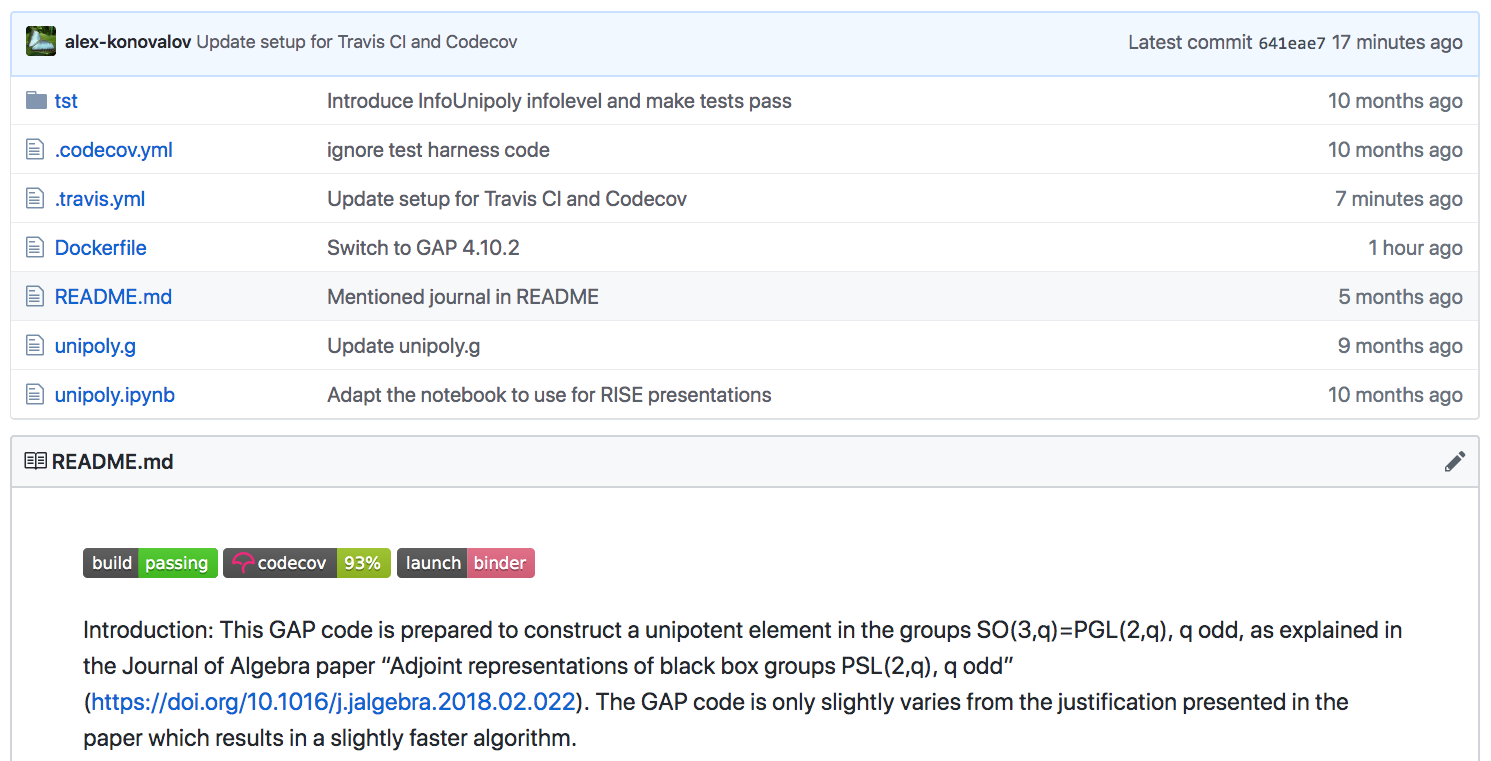
\includegraphics[width=\textwidth]{images/unipoly-repo}
    \caption{unipoly project repository}
    \label{fig:unipoly-repo}
\end{figure}

The next step is to produce a Jupyter notebook which combines input,
output, and textual narrative in one document. The notebook contains
the {\tt Read(unipoly.g);} command to read the code first. This is
a good practice for organising reproducible experiments: keeping the
code in a single location in a {\tt .g} file allows its reuse and
automated testing, and avoids code duplication. 

When the authors prepared and committed the Jupyter notebook describing
their calculation, they are ready to share it on
\href{https://mybinder.org/}{Binder}. First they need to add 
to their repository a {\tt Dockefile} with the following content:

\begin{figure}[!ht]
    \centering
    {\Small
\begin{verbatim}
FROM gapsystem/gap-docker

MAINTAINER Alexander Konovalov <alexander.konovalov@st-andrews.ac.uk>

COPY --chown=1000:1000 . $HOME/unipoly

RUN sudo pip3 install ipywidgets RISE

RUN jupyter-nbextension install rise --user --py

RUN jupyter-nbextension enable rise --user --py

USER gap

WORKDIR $HOME/unipoly
\end{verbatim}
    }
    \caption{Docker file for Binder.}
    \label{fig:pkgman-sample}
\end{figure}

This file builds a Docker container based on the container {\tt gapsystem/gap-docker}
with the latest \GAP release
(see Subsection~\ref{docker}). Additional commands specify how to copy the code into
the new container, and install additional extensions for Jupyter-based slideshows.

After that one should follow \href{https://mybinder.org/}{Binder} instructions to
set up a new Binder project. A completed setup will allow to click on the ``launch binder''
button in the README file on GitHub (as seen on Figure~\ref{fig:unipoly-repo}
to start a Jupyter notebook server in the cloud,
either using a prebuilt image of the project or by building a new one in case of any
changes in the GitHub repository. When the server will be started, it will display
a file browser as shown on Figure~\ref{fig:unipoly-files}.

\begin{figure}[!ht]
    \centering
    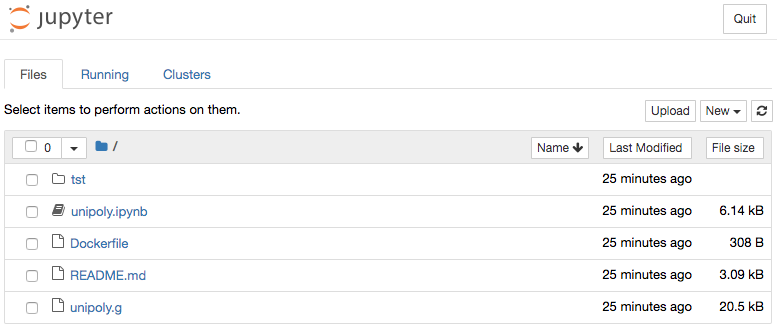
\includegraphics[width=\textwidth]{images/unipoly-files}
    \caption{File browser running on Binder}
    \label{fig:unipoly-files}
\end{figure}

Clicking on {\tt unipoly.ipynb}, the user will open the Jupyter notebook
and will be able to rerun it as shown on Figure~\ref{fig:unipoly-notebook}.

\begin{figure}[!ht]
    \centering
    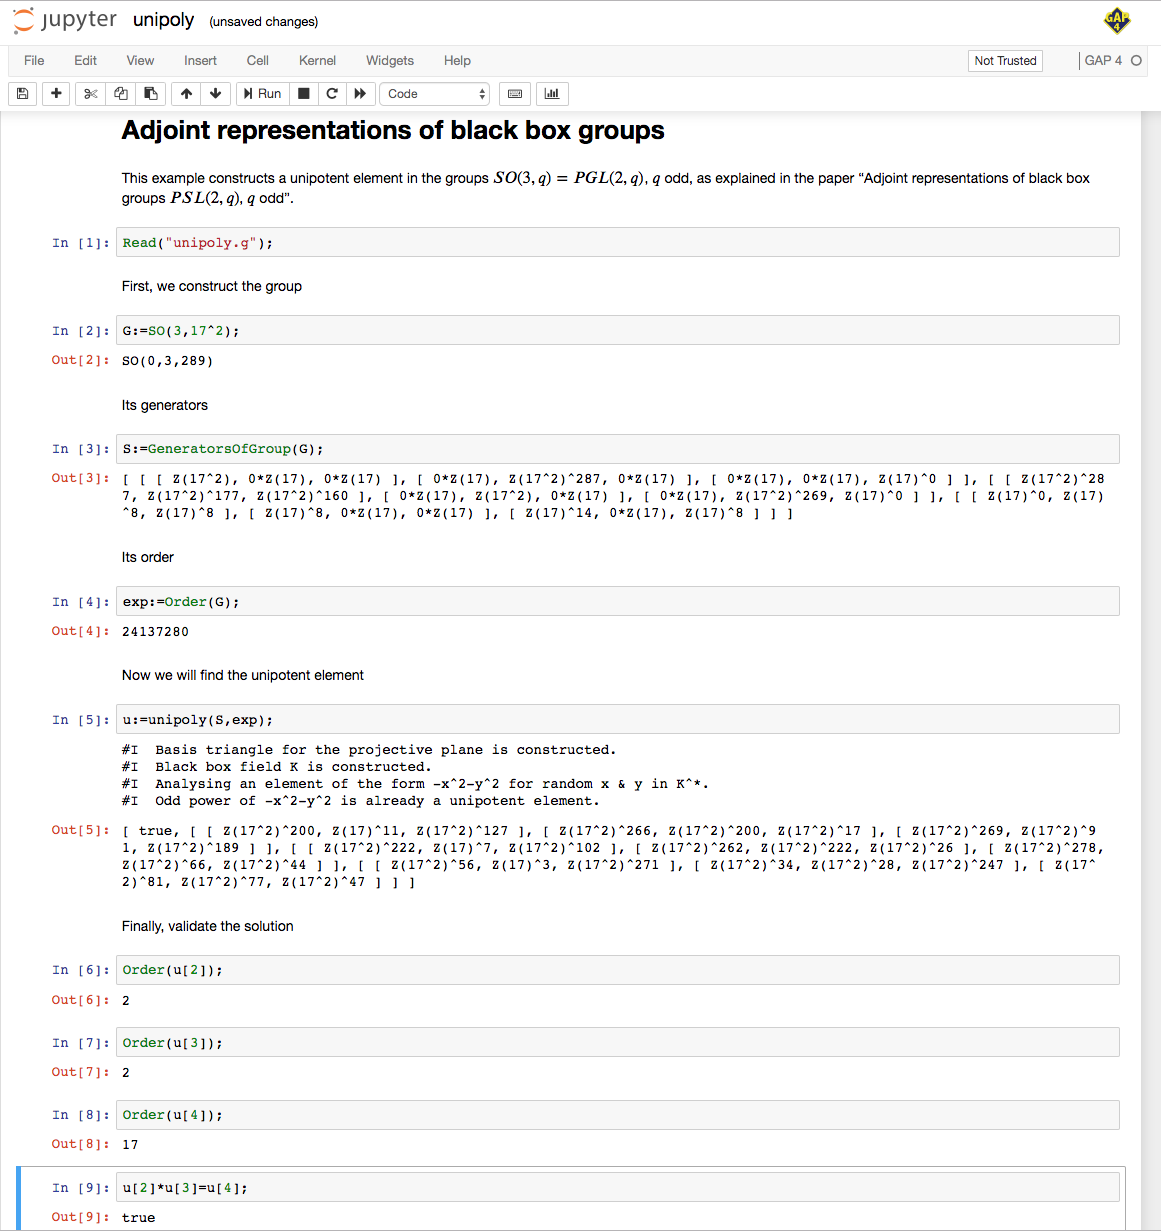
\includegraphics[width=\textwidth]{images/unipoly-notebook}
    \caption{Jupyter notebook running on Binder}
    \label{fig:unipoly-notebook}
\end{figure}

One could also switch to the slideshow mode (the notebook would require
some configuration to explain which cells should be displayed on the
same slide and which not), and run an interactive presentation, as
as shown on Figure~\ref{fig:unipoly-slide}.

\begin{figure}[!ht]
    \centering
    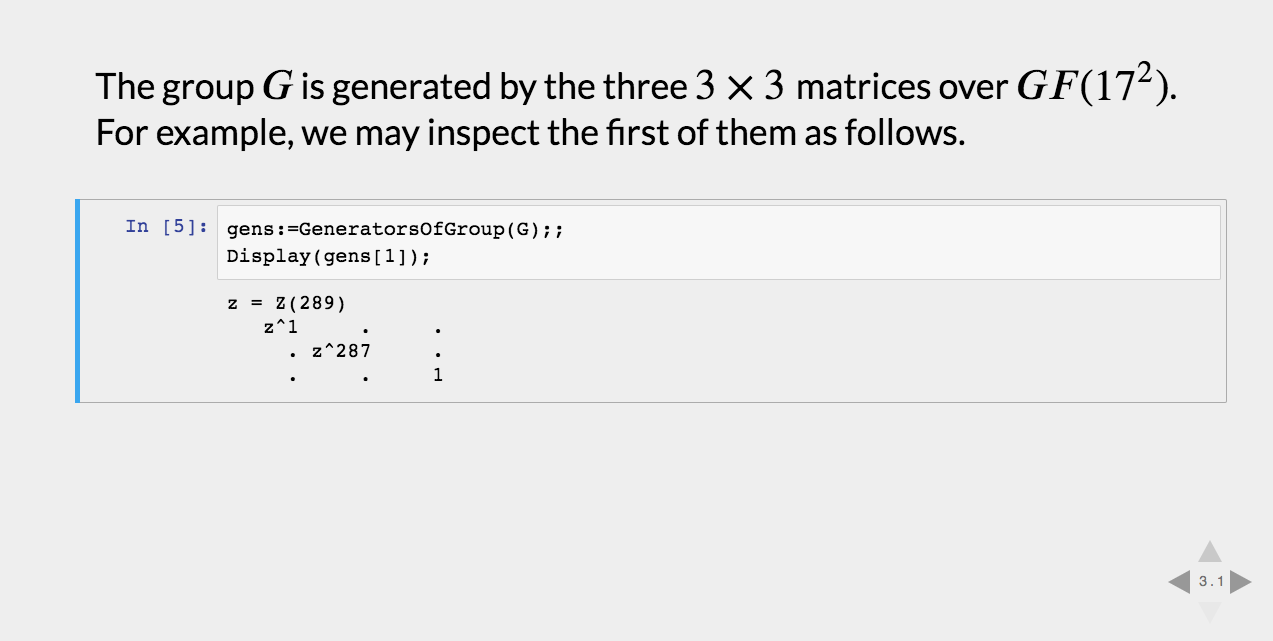
\includegraphics[width=\textwidth]{images/unipoly-slide}
    \caption{Slideshow with interactive computation running on Binder}
    \label{fig:unipoly-slide}
\end{figure}

Thus, connecting the project repository to Binder allows other users
(e.g. readers or referees of the paper) to rerun computations on Binder
without spending efforts on installing all necessary components
(may be hard for them as non experts, may not always be possible;
something may not work on Windows, etc.

\TODO{what are the limitations of Binder and suggested workarounds}


\clearpage
\TODO{Ensure that we are following software citation recommendations properly!}
\TODO{Can we break long URLs in the bibliography?}
\printbibliography

\end{document}


%%% Local Variables:
%%% mode: latex
%%% TeX-master: t
%%% End:

